\newpage
\section{Multilayer Perceptrons: Learned Nonlinear Representations}
\label{sec:multilayer-perceptrons}

This section evaluates a feed-forward multilayer perceptron (MLP) for churn prediction. An MLP extends a linear classifier by learning intermediate nonlinear feature transformations before it constructs the final churn score. This makes the model capable of representing interactions and nonlinear decision surfaces that would not be available to an ordinary additive logistic-regression specification without manually engineered interaction or basis features.

The held-out test set is not used anywhere in this section. Candidate architectures, regularization strengths, activation diagnostics, threshold curves, calibration diagnostics, and comparisons are produced from the training set only through the project's stratified cross-validation design. The reported configuration is therefore a development-stage candidate, not a final globally optimized neural network and not a final estimate of test performance. This maintains the train--validation--test separation used throughout the project \cite{ml-evaluation,dl-tools}.

\subsection{From logistic regression to learned nonlinear features}

For a transformed feature vector \(x\in\mathbb{R}^{d}\), logistic regression constructs one affine score
\[
\eta(x)=w^\top x+b
\]
and converts it into a churn probability through the sigmoid function
\[
\widehat{p}(x)=\sigma(\eta(x))
=
\frac{1}{1+\exp\{-\eta(x)\}}.
\]
The resulting boundary is linear in the transformed input space. One-hot encoded indicators permit different categorical groups to have different additive effects, but the model cannot automatically create arbitrary interactions such as a particular combination of contract type, internet service, tenure, and monthly charge.

An MLP instead learns hidden representations. For a network with \(L\) hidden layers, let \(h^{(0)}=x\). Each hidden layer applies an affine transformation followed by an element-wise nonlinearity:
\[
z^{(\ell)}
=
W^{(\ell)}h^{(\ell-1)}+b^{(\ell)},
\qquad
h^{(\ell)}
=
\phi\!\left(z^{(\ell)}\right),
\qquad
\ell=1,\ldots,L.
\]
The binary output layer produces a logit
\[
\eta(x)
=
w_{\mathrm{out}}^\top h^{(L)}+b_{\mathrm{out}},
\]
followed by
\[
\widehat{p}(x)
=
\sigma\!\left(\eta(x)\right).
\]

The activation function is essential. If every layer were affine, then the composition of layers would remain affine:
\[
W^{(2)}(W^{(1)}x+b^{(1)})+b^{(2)}
=
\underbrace{W^{(2)}W^{(1)}}_{\widetilde{W}}x
+
\underbrace{W^{(2)}b^{(1)}+b^{(2)}}_{\widetilde{b}}.
\]
Thus, stacking linear layers without nonlinear activation would not increase the functional class beyond a single linear model. The nonlinear transformation \(\phi\) permits the network to learn nonlinear representations.

\subsection{Hidden units, ReLU activations, and network capacity}

The principal candidates use the rectified linear unit,
\[
\operatorname{ReLU}(a)
=
\max\{0,a\}.
\]
ReLU creates a piecewise-linear nonlinear representation. It is computationally simple and avoids the severe saturation that can occur with sigmoid activations in hidden layers. A small \(\tanh\) diagnostic is also evaluated:
\[
\tanh(a)
=
\frac{\exp(a)-\exp(-a)}{\exp(a)+\exp(-a)}.
\]
Unlike ReLU, \(\tanh\) is bounded between \(-1\) and \(1\), which can be useful in some settings but may create smaller gradients when units saturate.

The selected architecture has one hidden layer with \(16\) ReLU units. The dense preprocessing pipeline produces \(46\) numeric input columns after fold-internal median imputation, standardization of numeric variables, and dense one-hot encoding of categorical variables. The number of trainable parameters is therefore
\[
(46+1)\times16+(16+1)\times1=769.
\]
The first term represents the hidden-layer weights and biases; the second represents the output-layer weights and bias. This is intentionally a modest capacity relative to the \(5{,}634\) training observations. Wider or deeper networks have more representational flexibility, but also more variance, more optimization sensitivity, and more opportunity to fit fold-specific idiosyncrasies.

\subsection{Binary cross-entropy and backpropagation}

The network is trained through the Bernoulli negative log-likelihood, commonly called binary cross-entropy:
\[
\mathcal{L}_{\mathrm{BCE}}
=
-\frac{1}{n}
\sum_{i=1}^{n}
\left[
y_i\log\widehat{p}_i
+
(1-y_i)\log(1-\widehat{p}_i)
\right].
\]
For a sigmoid output and binary cross-entropy, the derivative of the loss with respect to the output logit takes the particularly simple form
\[
\frac{\partial \mathcal{L}_{\mathrm{BCE}}}{\partial \eta_i}
=
\widehat{p}_i-y_i.
\]
Backpropagation applies the chain rule from this output error through the network. Writing \(\delta^{(L+1)}=\widehat{p}-y\) for the output error, the hidden-layer errors are propagated recursively:
\[
\delta^{(\ell)}
=
\left(W^{(\ell+1)\top}\delta^{(\ell+1)}\right)
\odot
\phi'\!\left(z^{(\ell)}\right).
\]
For a mini-batch of size \(m\), the gradient for a weight matrix is proportional to
\[
\nabla_{W^{(\ell)}}\mathcal{L}
=
\frac{1}{m}\delta^{(\ell)}h^{(\ell-1)\top}.
\]
The optimizer then updates every weight and bias in the direction that lowers the loss.

The implementation uses the Adam optimizer. Adam maintains running estimates of the first and second moments of the gradients and rescales updates coordinate by coordinate. This is convenient for a tabular model with a mixture of standardized continuous inputs and sparse one-hot indicators, but it does not remove the need for validation-based regularization and careful comparison.

\subsection{Regularization, early stopping, and leakage-safe preprocessing}

The MLP uses an L2 penalty, controlled by scikit-learn's \texttt{alpha} parameter:
\[
\mathcal{L}_{\mathrm{regularized}}
=
\mathcal{L}_{\mathrm{BCE}}
+
\frac{\alpha}{2n}\sum_{\ell}\left\lVert W^{(\ell)}\right\rVert_F^2.
\]
A larger \(\alpha\) shrinks weights more strongly and can reduce variance, while an overly large value may suppress useful structure.

Every MLP candidate is an sklearn pipeline. Numeric imputers, standardization parameters, category levels, and one-hot mappings are fitted only on each outer cross-validation training fold. This is necessary because neural networks are sensitive to numeric scale and because fitting preprocessing once on the complete training set would leak validation-fold distributional information into each fold's model.

The \texttt{MLPClassifier} candidates also use internal early stopping. Within an outer training fold, the classifier reserves \(15\%\) of that fold for its own internal validation split and stops after \(20\) iterations without an improvement in its internal validation accuracy. The outer-fold PR-AUC remains the model-selection metric. Internal validation accuracy is a training-control diagnostic, not the primary business or model-family selection criterion.

\subsection{Training-only search design}

The workflow uses a deliberately compact staged search rather than an exhaustive neural-network sweep. The initial shallow ReLU grid evaluates widths \(16\), \(32\), and \(64\), crossed with L2 strengths
\[
\alpha\in\{0.0001,0.001,0.01\}.
\]
The widths are geometrically spaced and the L2 values are logarithmically spaced. This is appropriate because a doubling of width or a tenfold change in a regularization scale is typically more meaningful than an arbitrary small additive change.

After the shallow grid, two two-hidden-layer architectures are evaluated using the strongest observed shallow-grid L2 value. Finally, the strongest ReLU architecture is compared with a \(\tanh\) version of the same architecture. This is a training-only development procedure, but it is not a fully predeclared Cartesian grid across every architecture, activation, and regularization combination. Consequently, small differences must not be interpreted as evidence of a uniquely optimal MLP.

\subsection{Shallow ReLU screen}

Table~\ref{tab:mlp-shallow-grid} reports the nine shallow ReLU candidates. The largest mean fold-level validation PR-AUC is \(0.6595\), achieved by the \(16\)-unit network with \(\alpha=0.001\). The \(16\)-unit alternatives are essentially tied: the difference between the selected configuration and the next candidate is only \(0.0007\), while their fold-level PR-AUC standard deviations are around \(0.018\)--\(0.019\).

The wider networks do not improve the main ranking metric. They also display larger train--validation PR-AUC gaps, especially for \(64\) hidden units. This pattern does not prove overfitting in a formal population sense, but it is consistent with extra capacity fitting the outer-fold training partitions more strongly without producing better validation ranking.

\begin{table}[H]
\centering
\small
\resizebox{\textwidth}{!}{
\begin{tabular}{lrrrrrrr}
\toprule
Hidden units & \(\alpha\) & Mean CV PR-AUC & SD & Mean CV ROC-AUC & Bal. Acc. & \(F_1\) & Train--valid. PR gap \\
\midrule
\(16\) & 0.0010 & 0.6595 & 0.0183 & 0.8436 & 0.7108 & 0.5798 & 0.0096 \\
\(16\) & 0.0100 & 0.6588 & 0.0189 & 0.8432 & 0.7126 & 0.5828 & 0.0099 \\
\(16\) & 0.0001 & 0.6586 & 0.0193 & 0.8428 & 0.7077 & 0.5748 & 0.0079 \\
\(32\) & 0.0100 & 0.6580 & 0.0215 & 0.8442 & 0.7206 & 0.5964 & 0.0215 \\
\(32\) & 0.0010 & 0.6576 & 0.0213 & 0.8440 & 0.7164 & 0.5890 & 0.0158 \\
\(32\) & 0.0001 & 0.6567 & 0.0208 & 0.8441 & 0.7152 & 0.5869 & 0.0172 \\
\(64\) & 0.0010 & 0.6567 & 0.0156 & 0.8423 & 0.7153 & 0.5876 & 0.0385 \\
\(64\) & 0.0100 & 0.6565 & 0.0158 & 0.8426 & 0.7204 & 0.5942 & 0.0302 \\
\(64\) & 0.0001 & 0.6559 & 0.0156 & 0.8425 & 0.7170 & 0.5902 & 0.0383 \\
\bottomrule
\end{tabular}
}
\caption{Shallow ReLU MLP screen using mean outer-fold validation metrics. The train--validation gap is mean train PR-AUC minus mean validation PR-AUC.}
\label{tab:mlp-shallow-grid}
\end{table}

\begin{figure}[H]
\centering
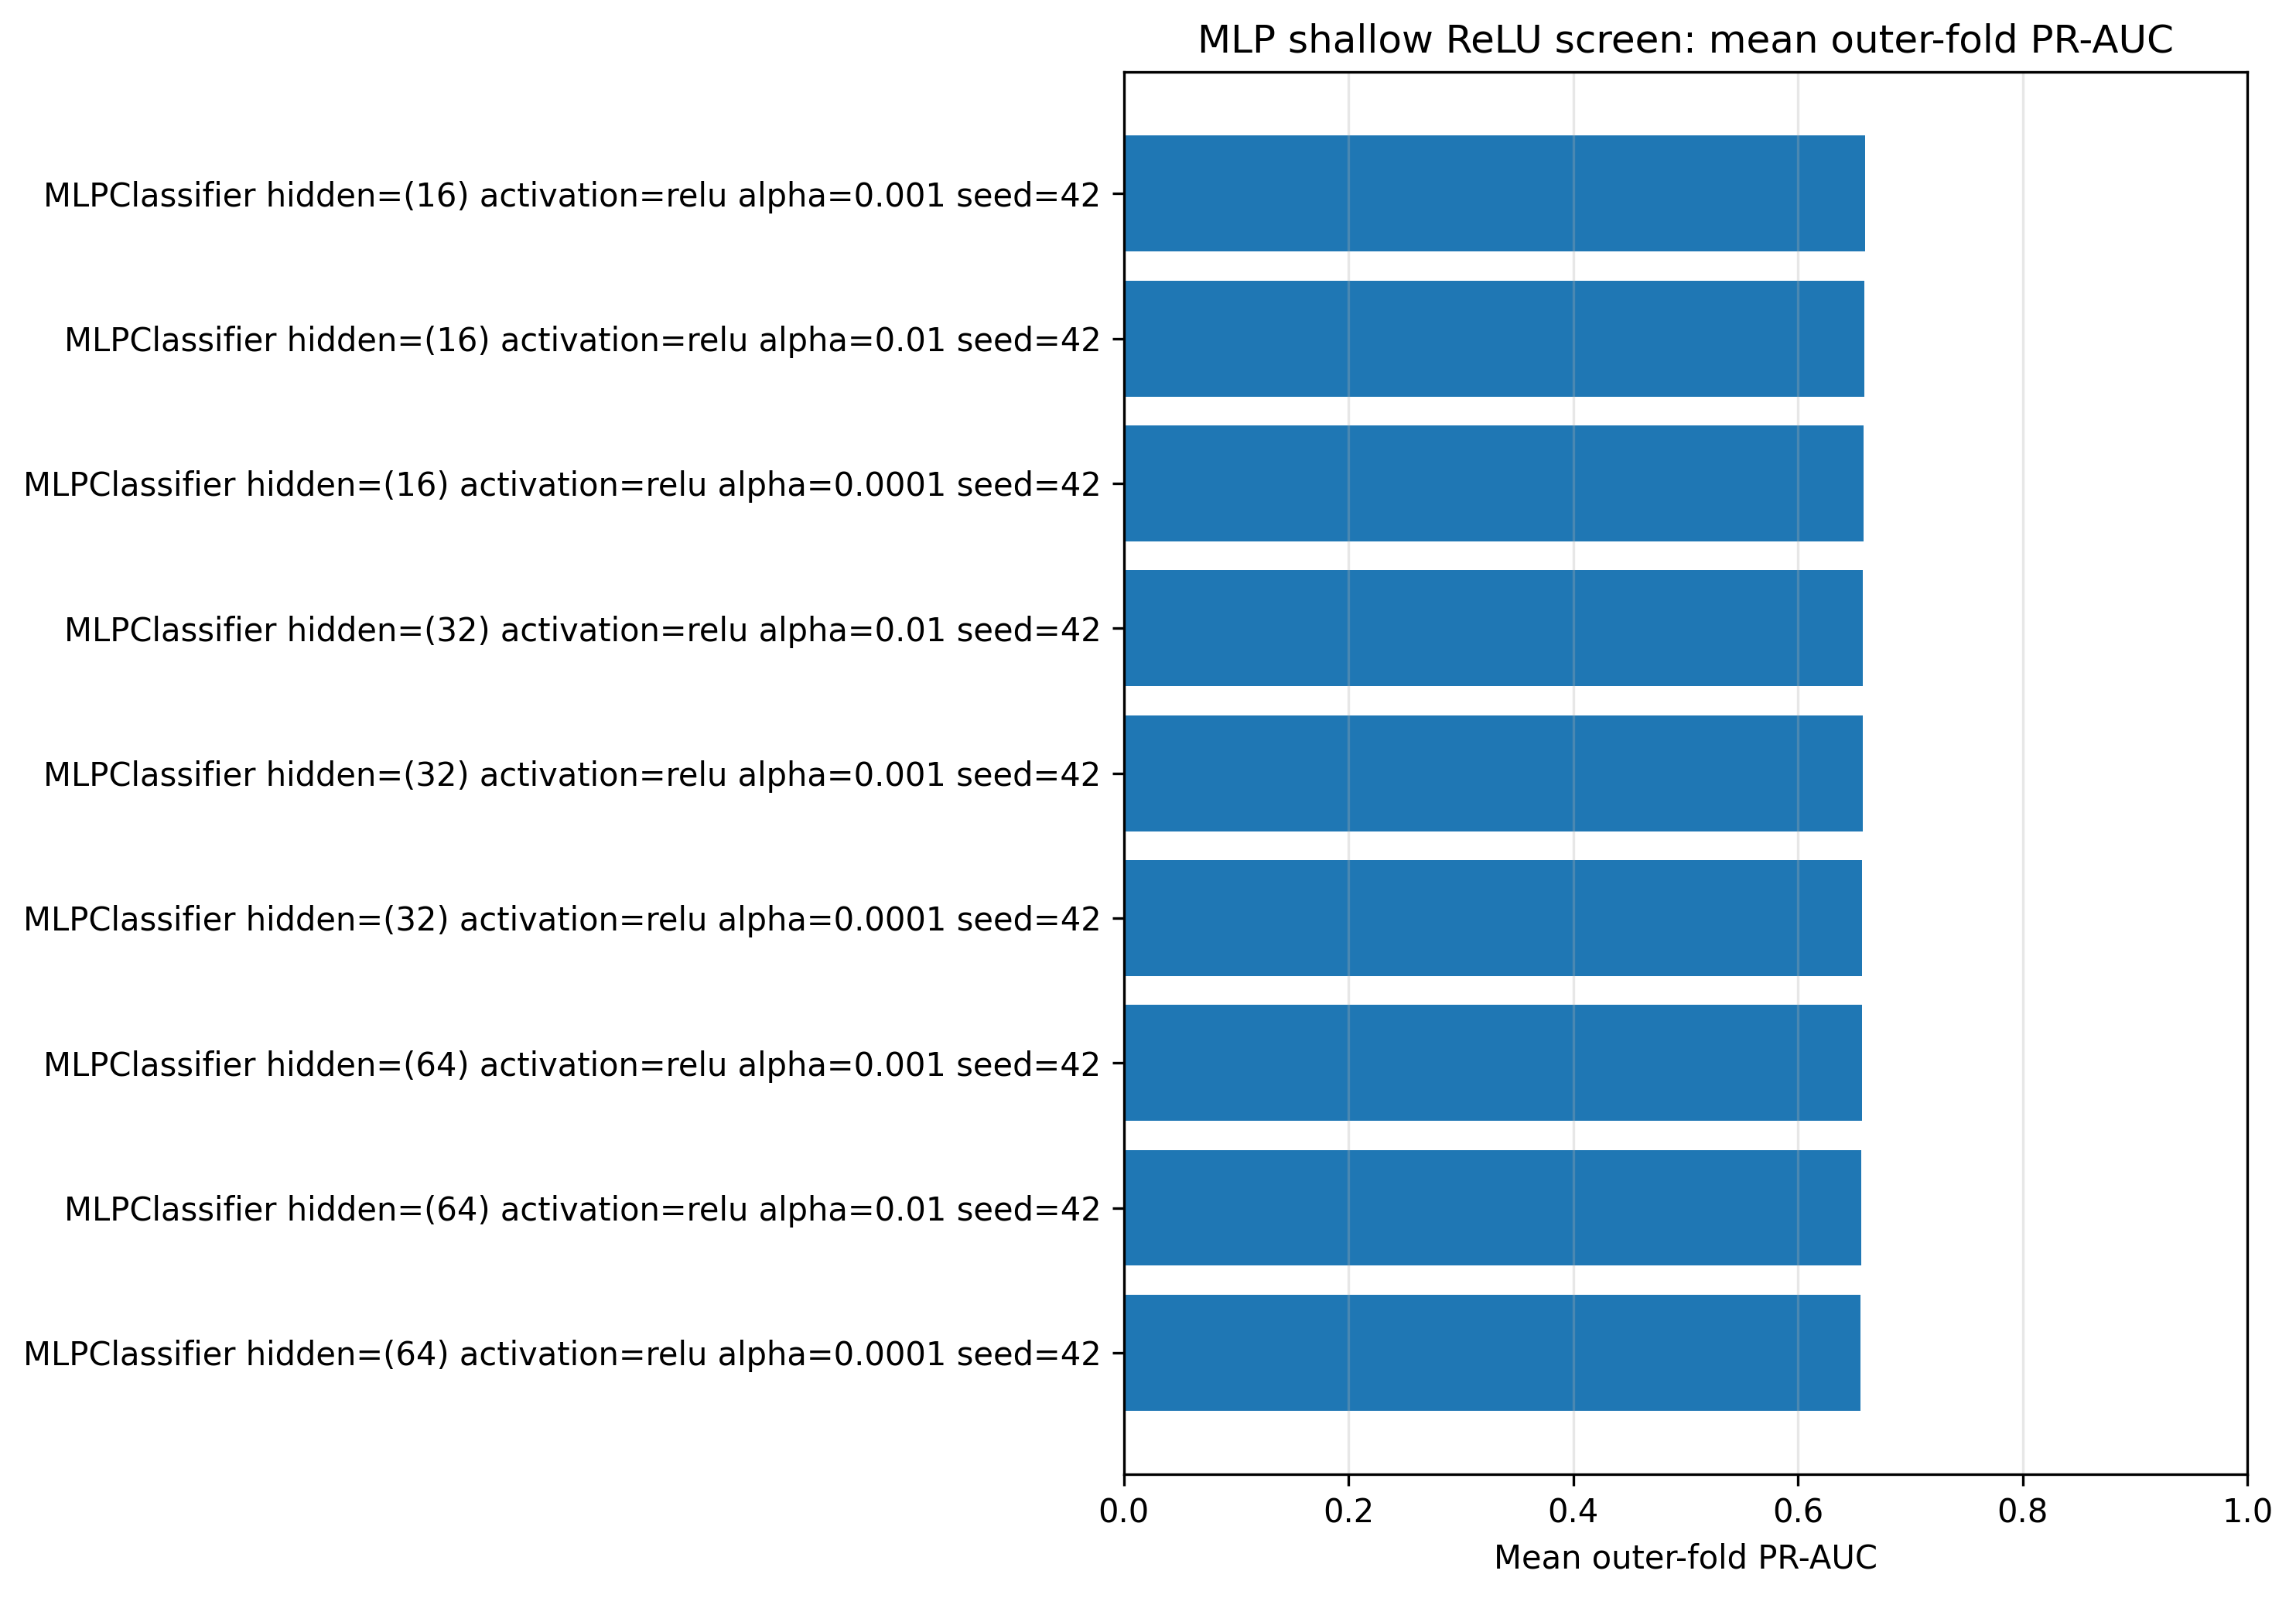
\includegraphics[width=0.90\textwidth]{../figures/mlp_shallow_grid_pr_auc.png}
\caption{Shallow ReLU MLP candidates ranked by mean outer-fold PR-AUC}
\label{fig:mlp-shallow-grid}
\end{figure}

\subsection{Depth and activation diagnostics}

Adding a second hidden layer does not improve the observed ranking quality. The \((64,32)\) architecture reaches mean CV PR-AUC \(0.6523\), while \((32,16)\) reaches \(0.6507\), both below the selected one-hidden-layer candidate. The \(\tanh\) version of the selected \(16\)-unit architecture reaches \(0.6559\), also below the ReLU result.

These diagnostics suggest that the available feature representation and sample size do not provide a visible benefit from additional depth or the alternative hidden activation. They do not imply that deep networks are universally unsuitable for tabular data. They only describe this compact candidate set on this dataset.

\begin{table}[H]
\centering
\small
\begin{tabular}{llrrrrr}
\toprule
Architecture & Activation & Mean CV PR-AUC & SD & Mean CV ROC-AUC & \(F_1\) & Train--valid. PR gap \\
\midrule
\(16\) & ReLU & 0.6595 & 0.0183 & 0.8436 & 0.5798 & 0.0096 \\
\((64,32)\) & ReLU & 0.6523 & 0.0196 & 0.8407 & 0.5891 & 0.0220 \\
\((32,16)\) & ReLU & 0.6507 & 0.0196 & 0.8444 & 0.5819 & 0.0275 \\
\(16\) & \(\tanh\) & 0.6559 & 0.0273 & 0.8409 & 0.5766 & 0.0062 \\
\bottomrule
\end{tabular}
\caption{Depth and activation diagnostics after the shallow ReLU screen}
\label{tab:mlp-depth-activation}
\end{table}

\begin{figure}[H]
\centering
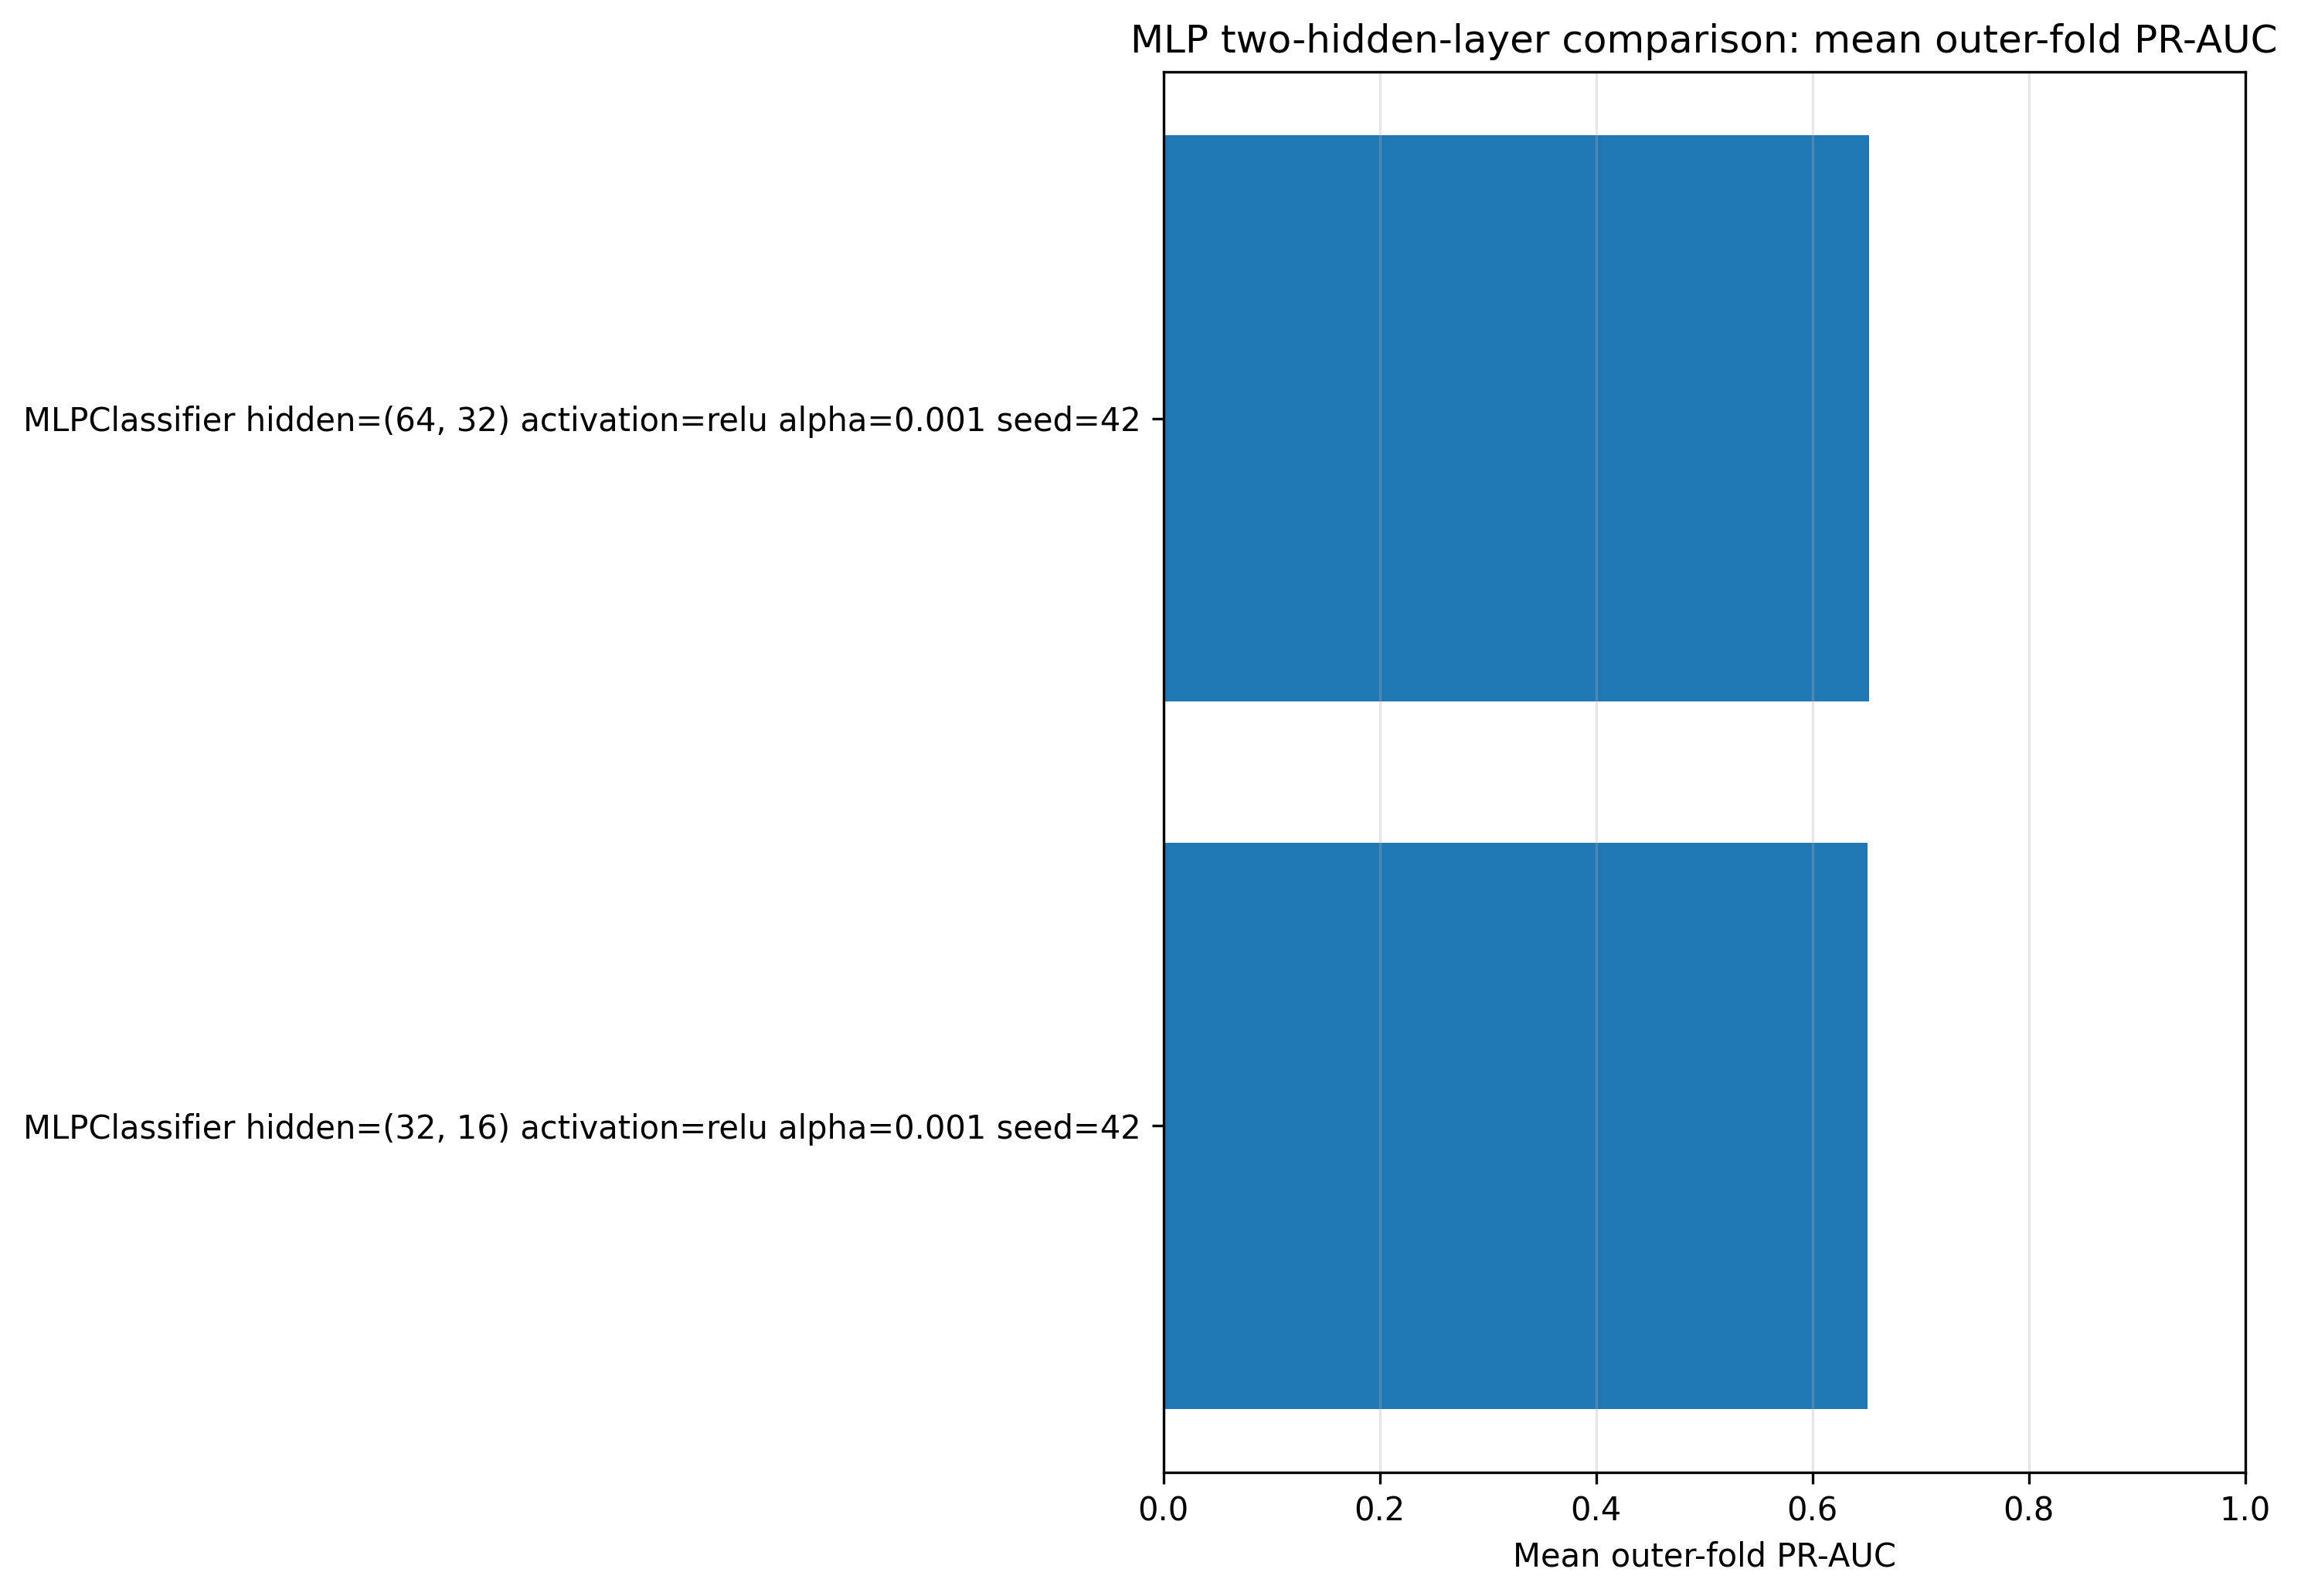
\includegraphics[width=0.84\textwidth]{../figures/mlp_depth_comparison_pr_auc.png}
\caption{Two-hidden-layer MLP diagnostic: mean outer-fold PR-AUC}
\label{fig:mlp-depth-comparison}
\end{figure}

\subsection{Selected MLP and pooled out-of-fold evaluation}

The development-stage representative is the one-hidden-layer ReLU network with \(16\) units and \(\alpha=0.001\). It was selected by mean outer-fold PR-AUC, followed by balanced accuracy and \(F_1\). Its grid-selection statistic is mean fold-level PR-AUC \(0.6595\). When one out-of-fold probability is concatenated for each training observation, the pooled OOF PR-AUC is \(0.6544\) and the pooled OOF ROC-AUC is \(0.8425\).

Mean fold-level PR-AUC and pooled OOF PR-AUC are different statistics. Average precision is nonlinear, and each fold is fitted independently. The mean fold-level score remains the pre-specified grid-selection statistic. The pooled OOF probabilities are used for common diagnostics such as the ROC curve, PR curve, calibration diagnostic, confusion matrix, and threshold analysis.

At the default probability threshold \(0.50\), the MLP identifies \(769\) of \(1495\) churners and produces \(384\) false positives. Its precision is \(0.667\), recall is \(0.514\), and specificity is \(0.907\). The model flags \(20.5\%\) of customers as likely churners, below the observed churn rate of \(26.5\%\). Thus, the unweighted default operating point is relatively conservative: it produces a selective list with good precision and specificity, but it misses nearly half of the observed churners.

\begin{table}[H]
\centering
\small
\begin{tabular}{lrrrrrrrr}
\toprule
Model & Accuracy & Bal. Acc. & Precision & Recall & Specificity & \(F_1\) & ROC-AUC & PR-AUC \\
\midrule
Selected MLP & 0.803 & 0.711 & 0.667 & 0.514 & 0.907 & 0.581 & 0.842 & 0.654 \\
\bottomrule
\end{tabular}
\caption{Pooled out-of-fold diagnostics for the selected MLP}
\label{tab:mlp-selected-oof}
\end{table}

\begin{table}[H]
\centering
\small
\begin{tabular}{rrrrr}
\toprule
TP & FN & FP & TN & Predicted positive rate \\
\midrule
769 & 726 & 384 & 3755 & 0.205 \\
\bottomrule
\end{tabular}
\caption{Positive-first pooled out-of-fold confusion-matrix counts for the selected MLP at threshold \(0.50\)}
\label{tab:mlp-confusion}
\end{table}

\begin{figure}[H]
\centering
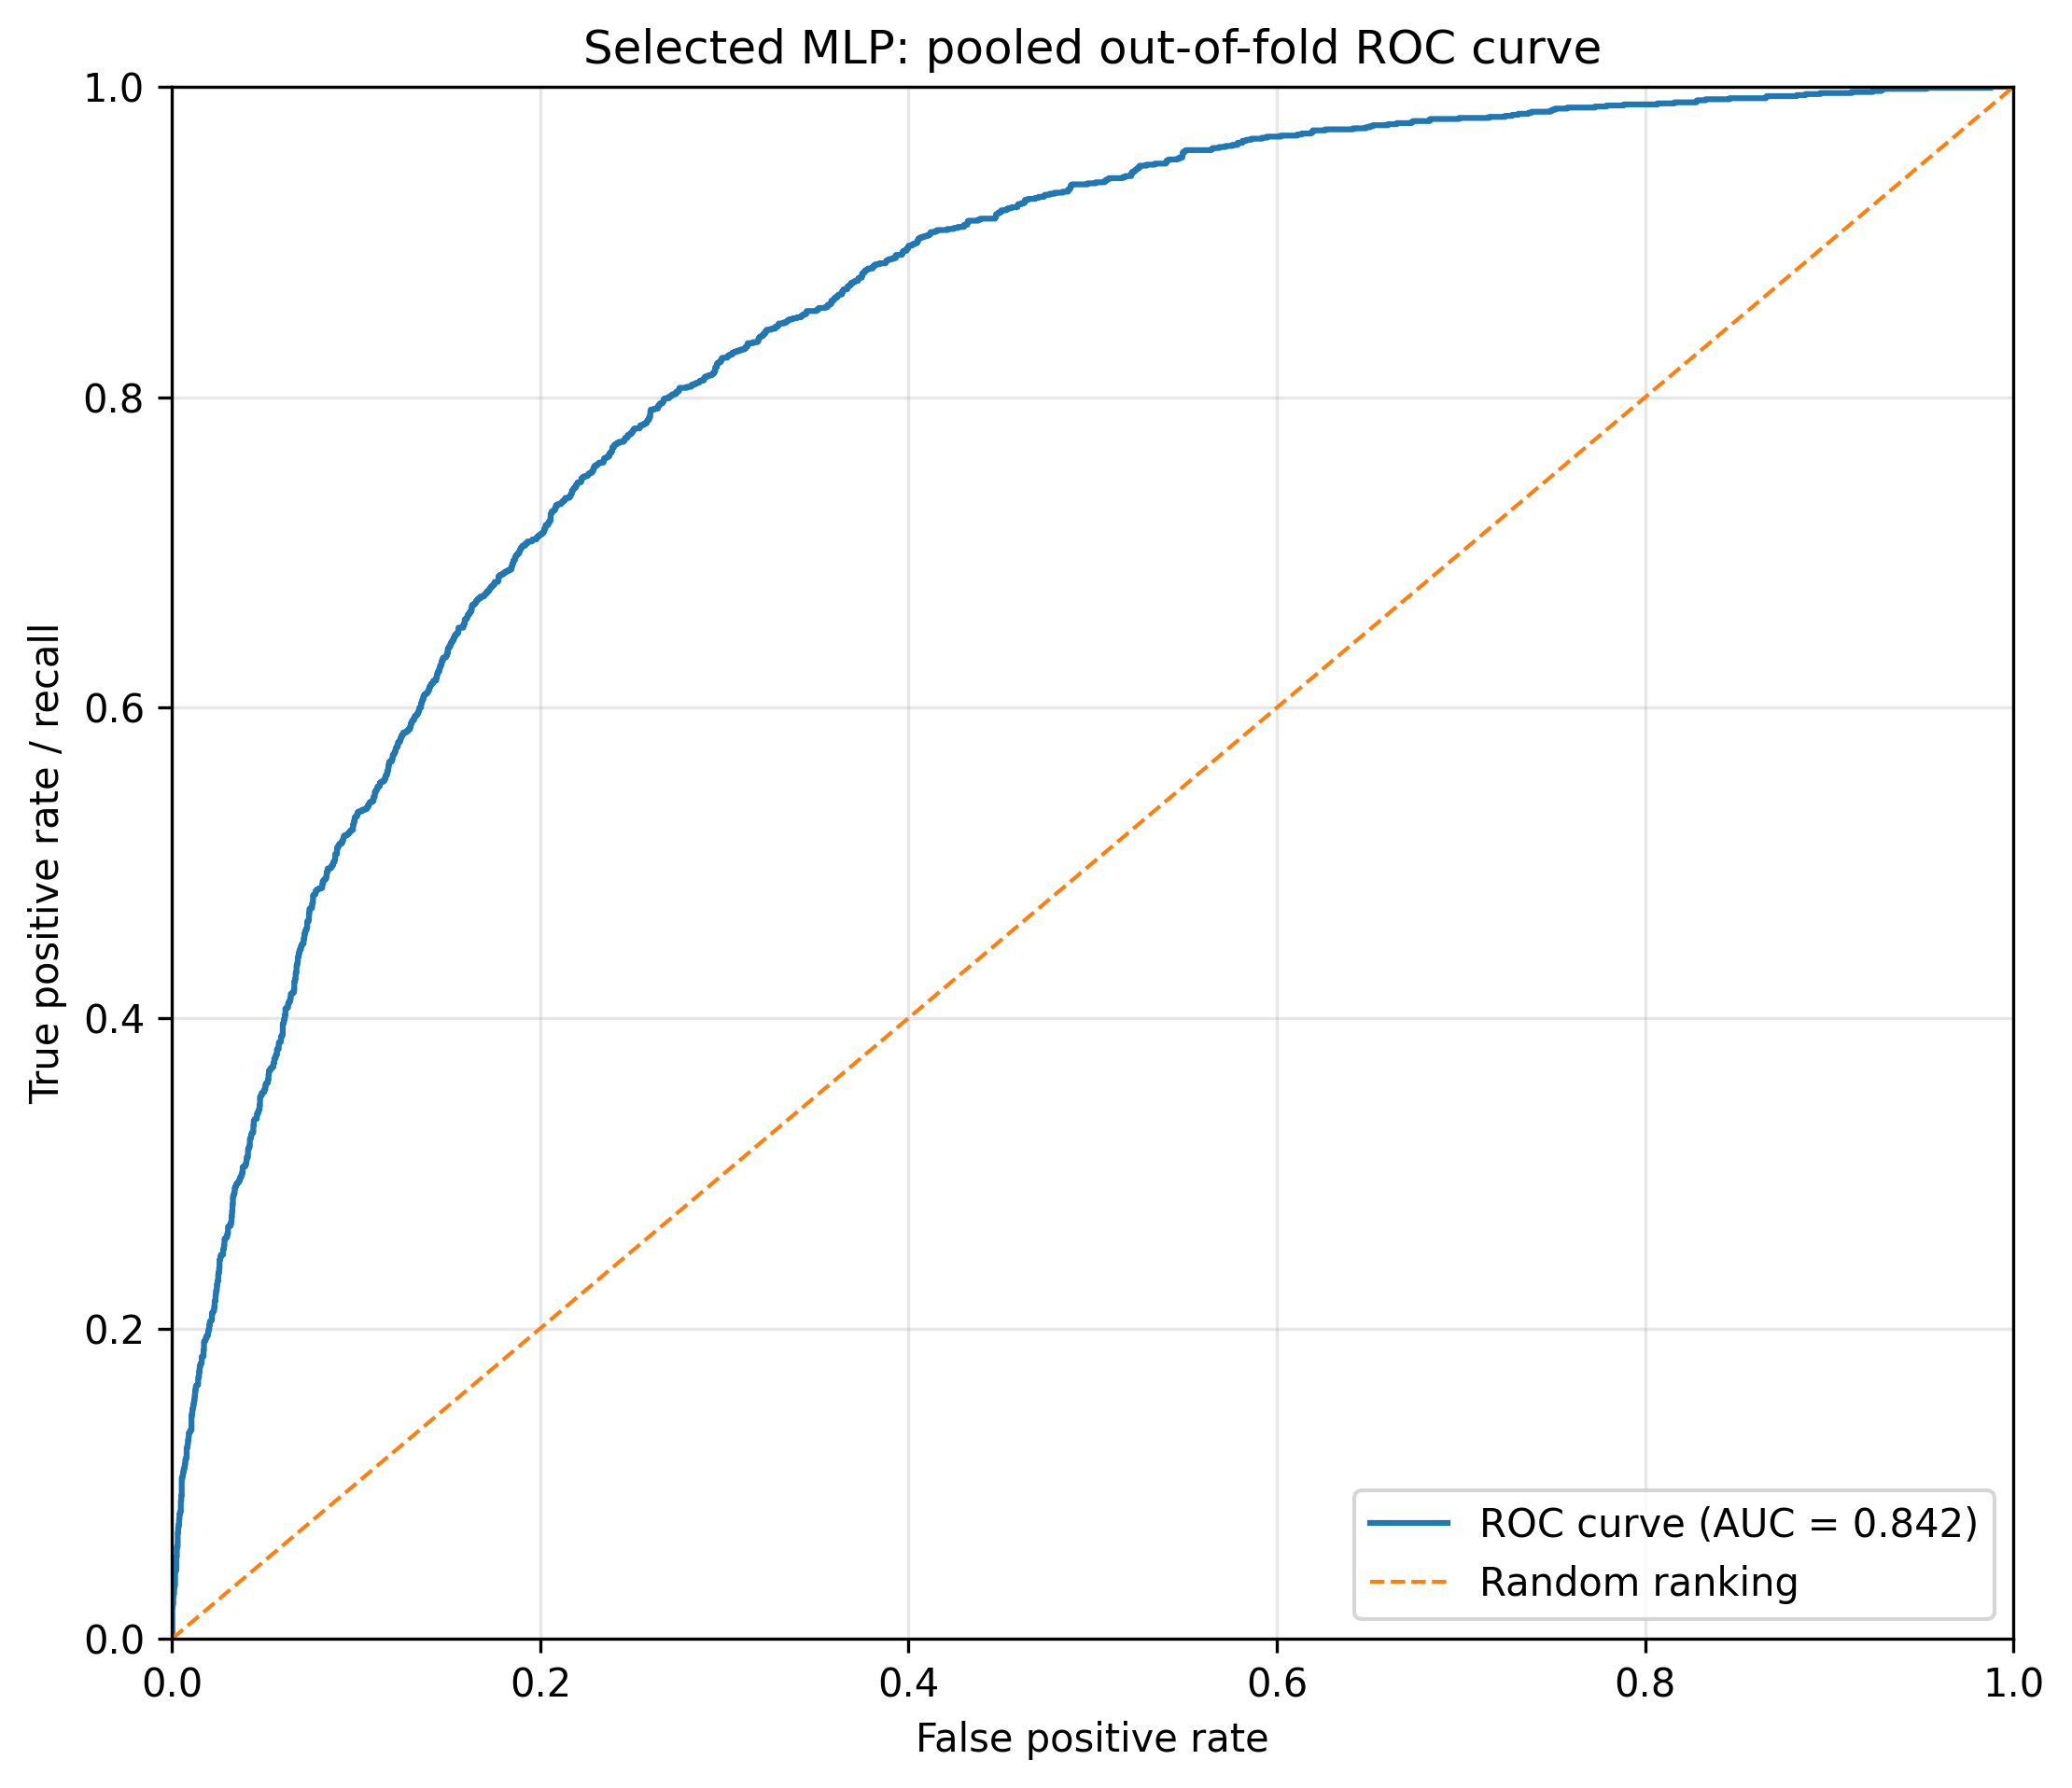
\includegraphics[width=0.82\textwidth]{../figures/mlp_roc_curve.png}
\caption{ROC curve for the selected MLP using pooled out-of-fold churn probabilities}
\label{fig:mlp-roc-curve}
\end{figure}

\begin{figure}[H]
\centering
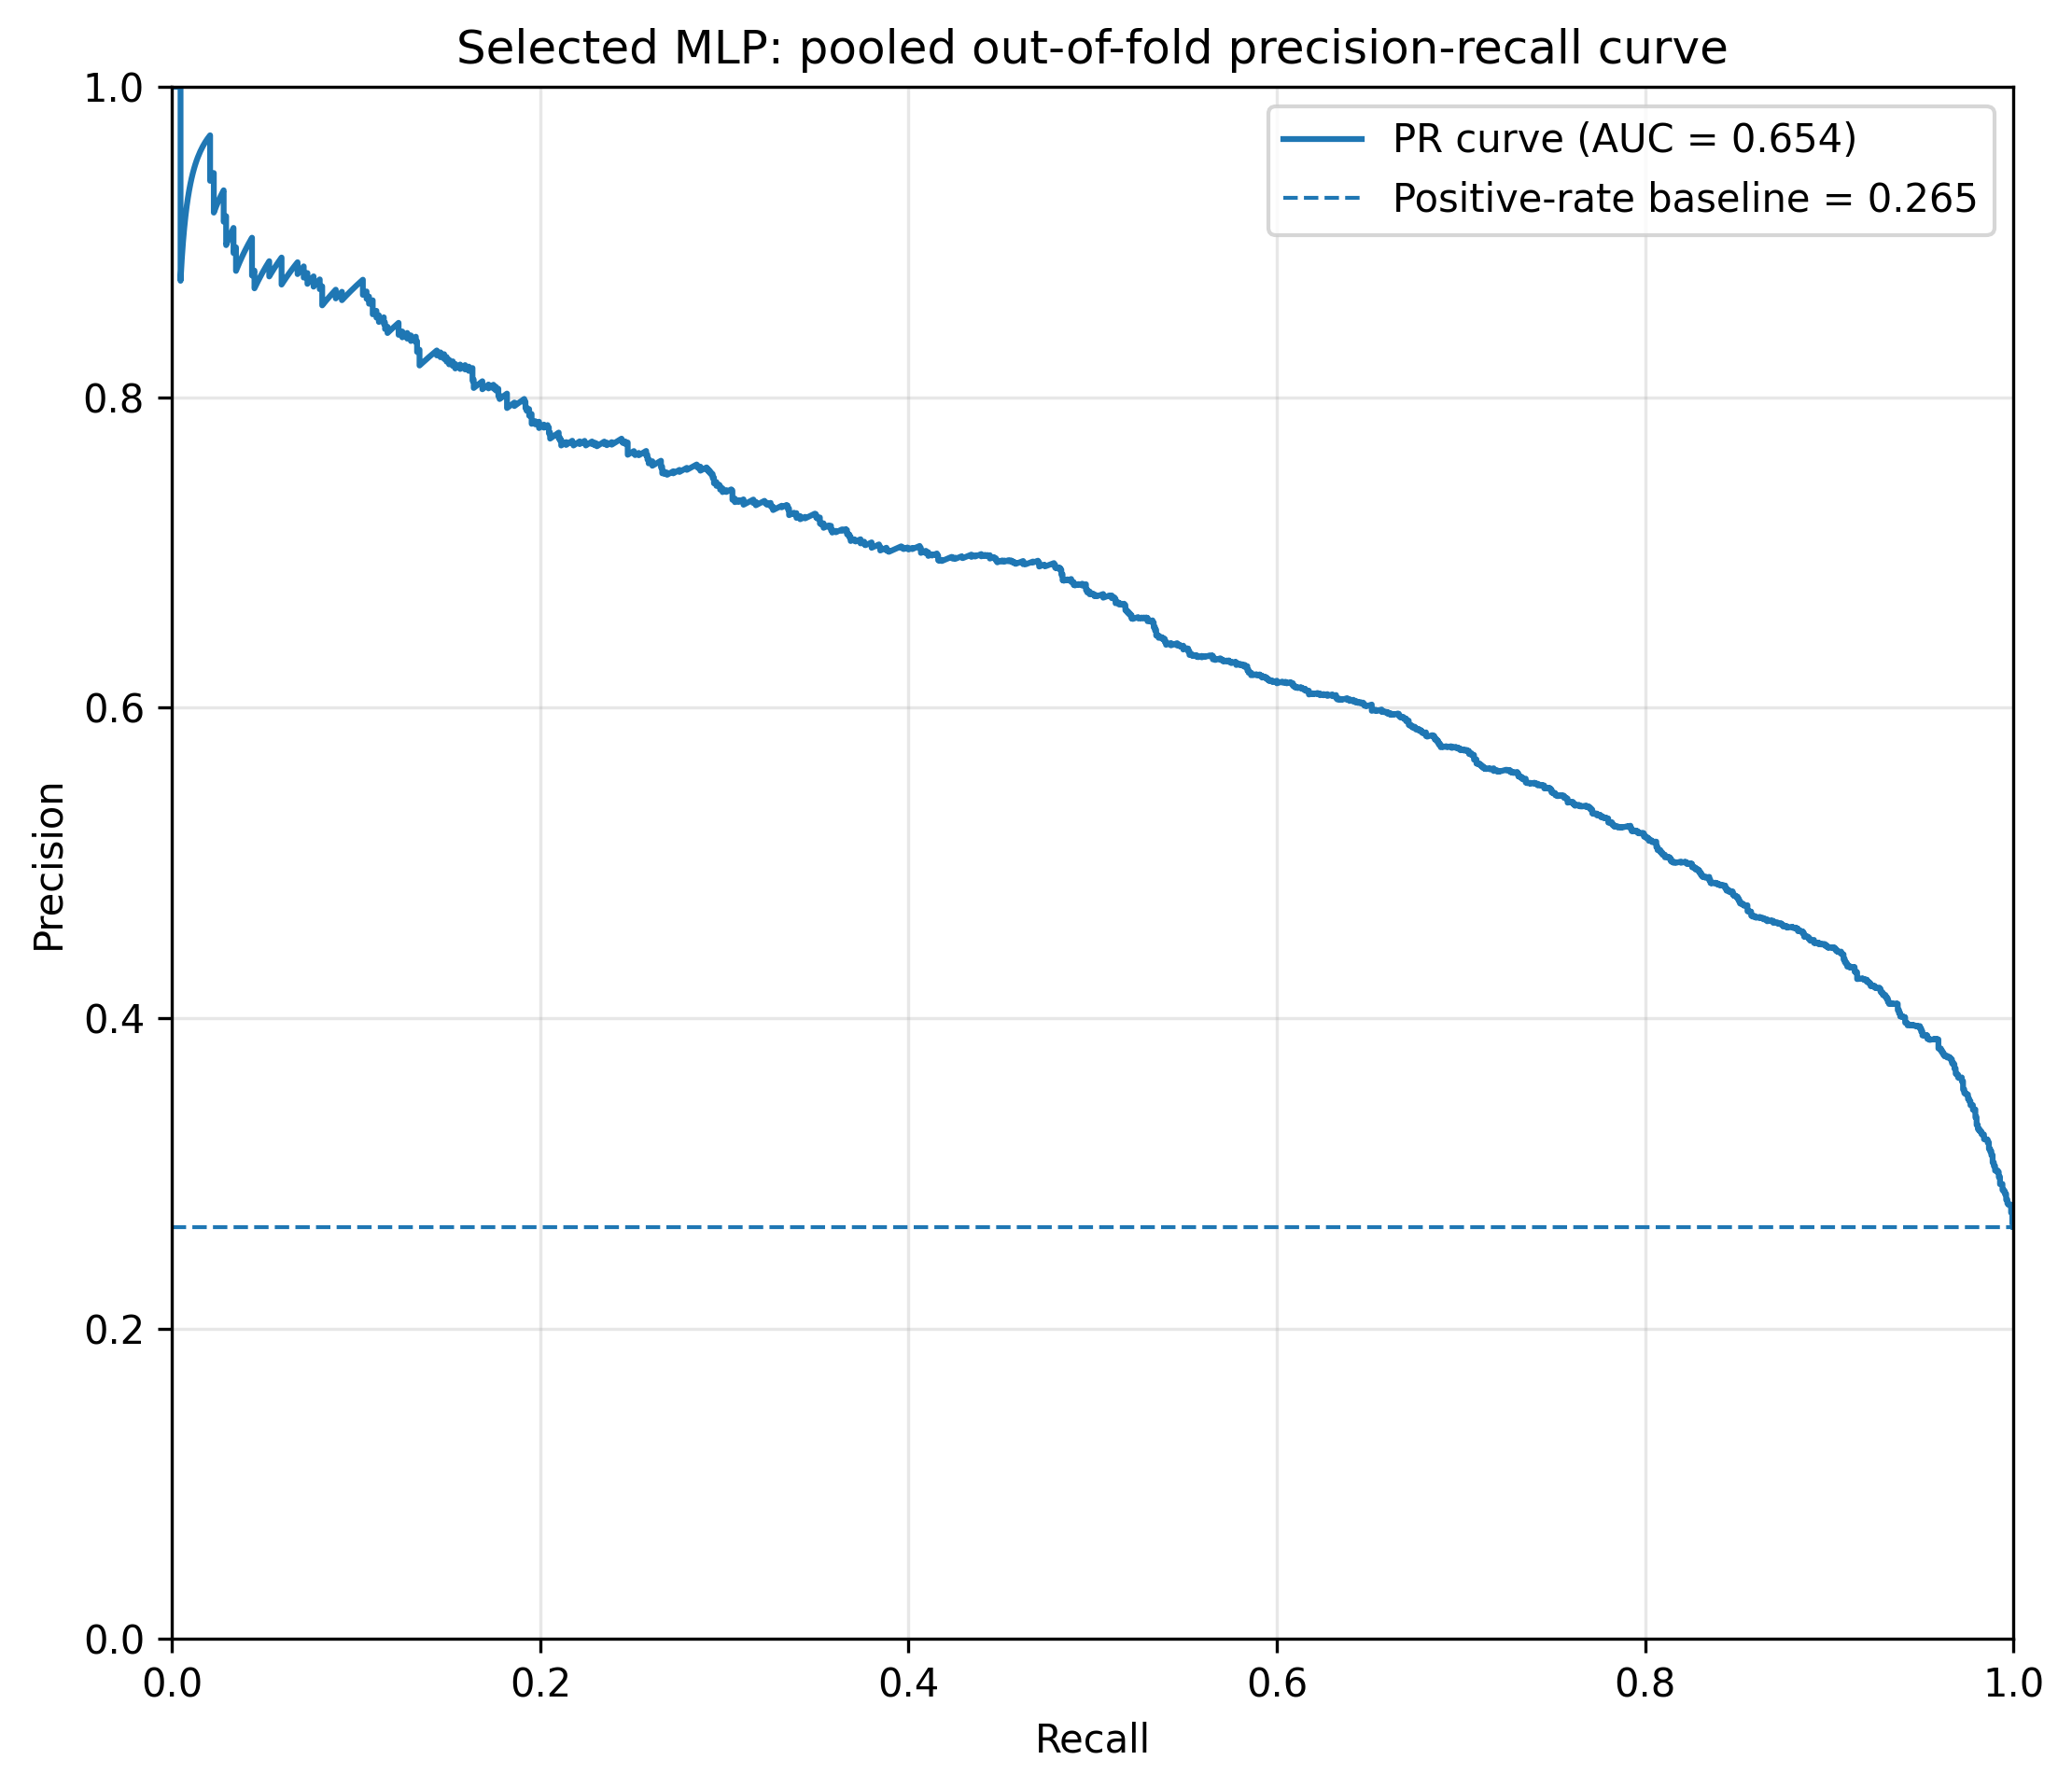
\includegraphics[width=0.82\textwidth]{../figures/mlp_precision_recall_curve.png}
\caption{Precision--recall curve for the selected MLP using pooled out-of-fold churn probabilities}
\label{fig:mlp-pr-curve}
\end{figure}

The PR curve remains materially above the positive-rate baseline of \(0.265\), showing useful churn-risk ranking. However, the observed PR-AUC does not establish a material nonlinear advantage over the project’s strong linear and tree-based references. That question requires fair finalist comparison after all model-family work is complete.

Figure~\ref{fig:mlp-probability-distribution} provides a complementary view of the score distribution. Observed churners are shifted toward larger predicted probabilities, whereas observed non-churners are concentrated near zero. The substantial overlap is expected in a realistic churn task and explains why no fixed threshold simultaneously obtains both very high precision and very high recall.

\begin{figure}[H]
\centering
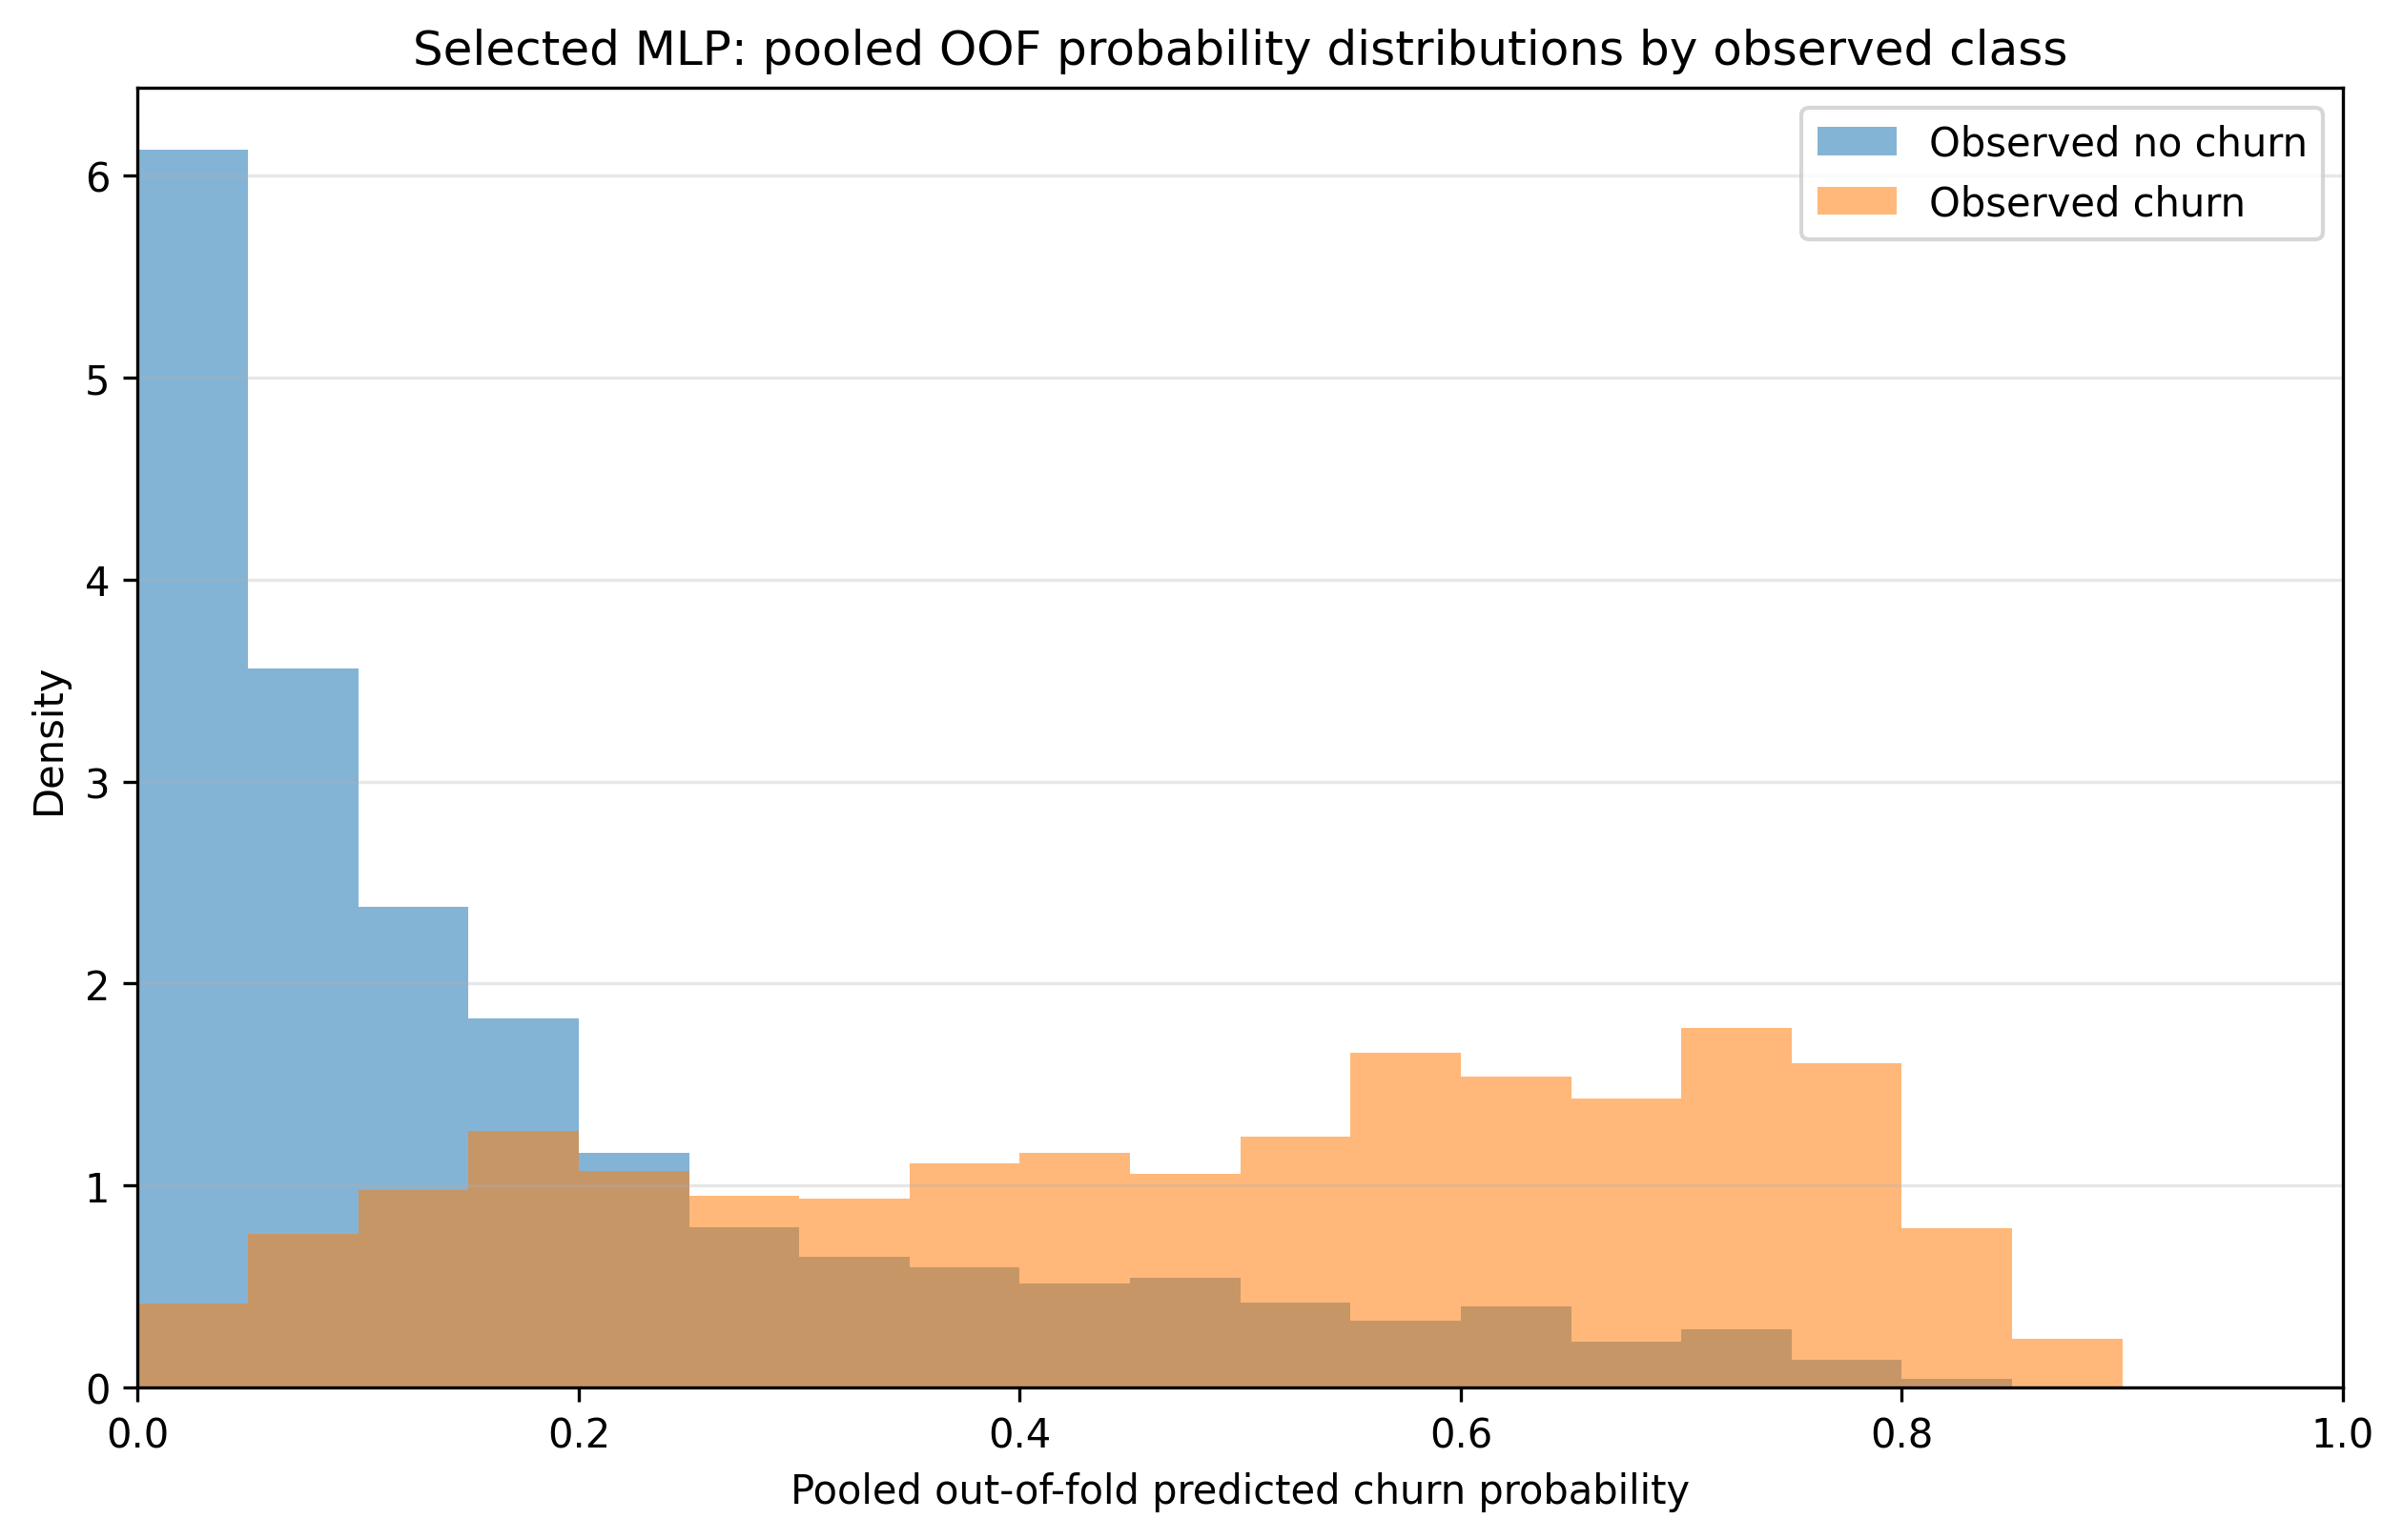
\includegraphics[width=0.88\textwidth]{../figures/mlp_oof_probability_distribution.png}
\caption{Pooled out-of-fold churn-probability distributions by observed class for the selected MLP}
\label{fig:mlp-probability-distribution}
\end{figure}

\subsection{Threshold behaviour and operating-point tradeoffs}

Because the MLP produces probabilities, its threshold has a direct operational interpretation only to the extent that calibration is adequate. Lowering the threshold identifies more potential churners, but increases the intervention list and false-positive rate. Table~\ref{tab:mlp-thresholds} shows selected thresholds calculated from the pooled OOF probabilities.

Within the displayed grid, a threshold of \(0.30\) has the largest \(F_1\), \(0.632\). A threshold of \(0.25\) has the largest displayed balanced accuracy, \(0.764\). Neither value should be adopted as a final production rule here. Both were inspected on the same training-only development evidence used for model selection, and the eventual threshold must depend on intervention capacity, retention value, and the relative cost of missed churners and unnecessary contacts.

\begin{table}[H]
\centering
\small
\begin{tabular}{rrrrrr}
\toprule
Threshold & Precision & Recall & Specificity & \(F_1\) & Pred. positive rate \\
\midrule
0.10 & 0.397 & 0.941 & 0.484 & 0.559 & 0.629 \\
0.20 & 0.495 & 0.829 & 0.695 & 0.620 & 0.444 \\
0.25 & 0.531 & 0.775 & 0.753 & 0.630 & 0.387 \\
0.30 & 0.559 & 0.728 & 0.792 & 0.632 & 0.346 \\
0.50 & 0.667 & 0.514 & 0.907 & 0.581 & 0.205 \\
0.65 & 0.751 & 0.292 & 0.965 & 0.421 & 0.103 \\
\bottomrule
\end{tabular}
\caption{Selected probability thresholds for the MLP using pooled out-of-fold predictions}
\label{tab:mlp-thresholds}
\end{table}

\begin{figure}[H]
\centering
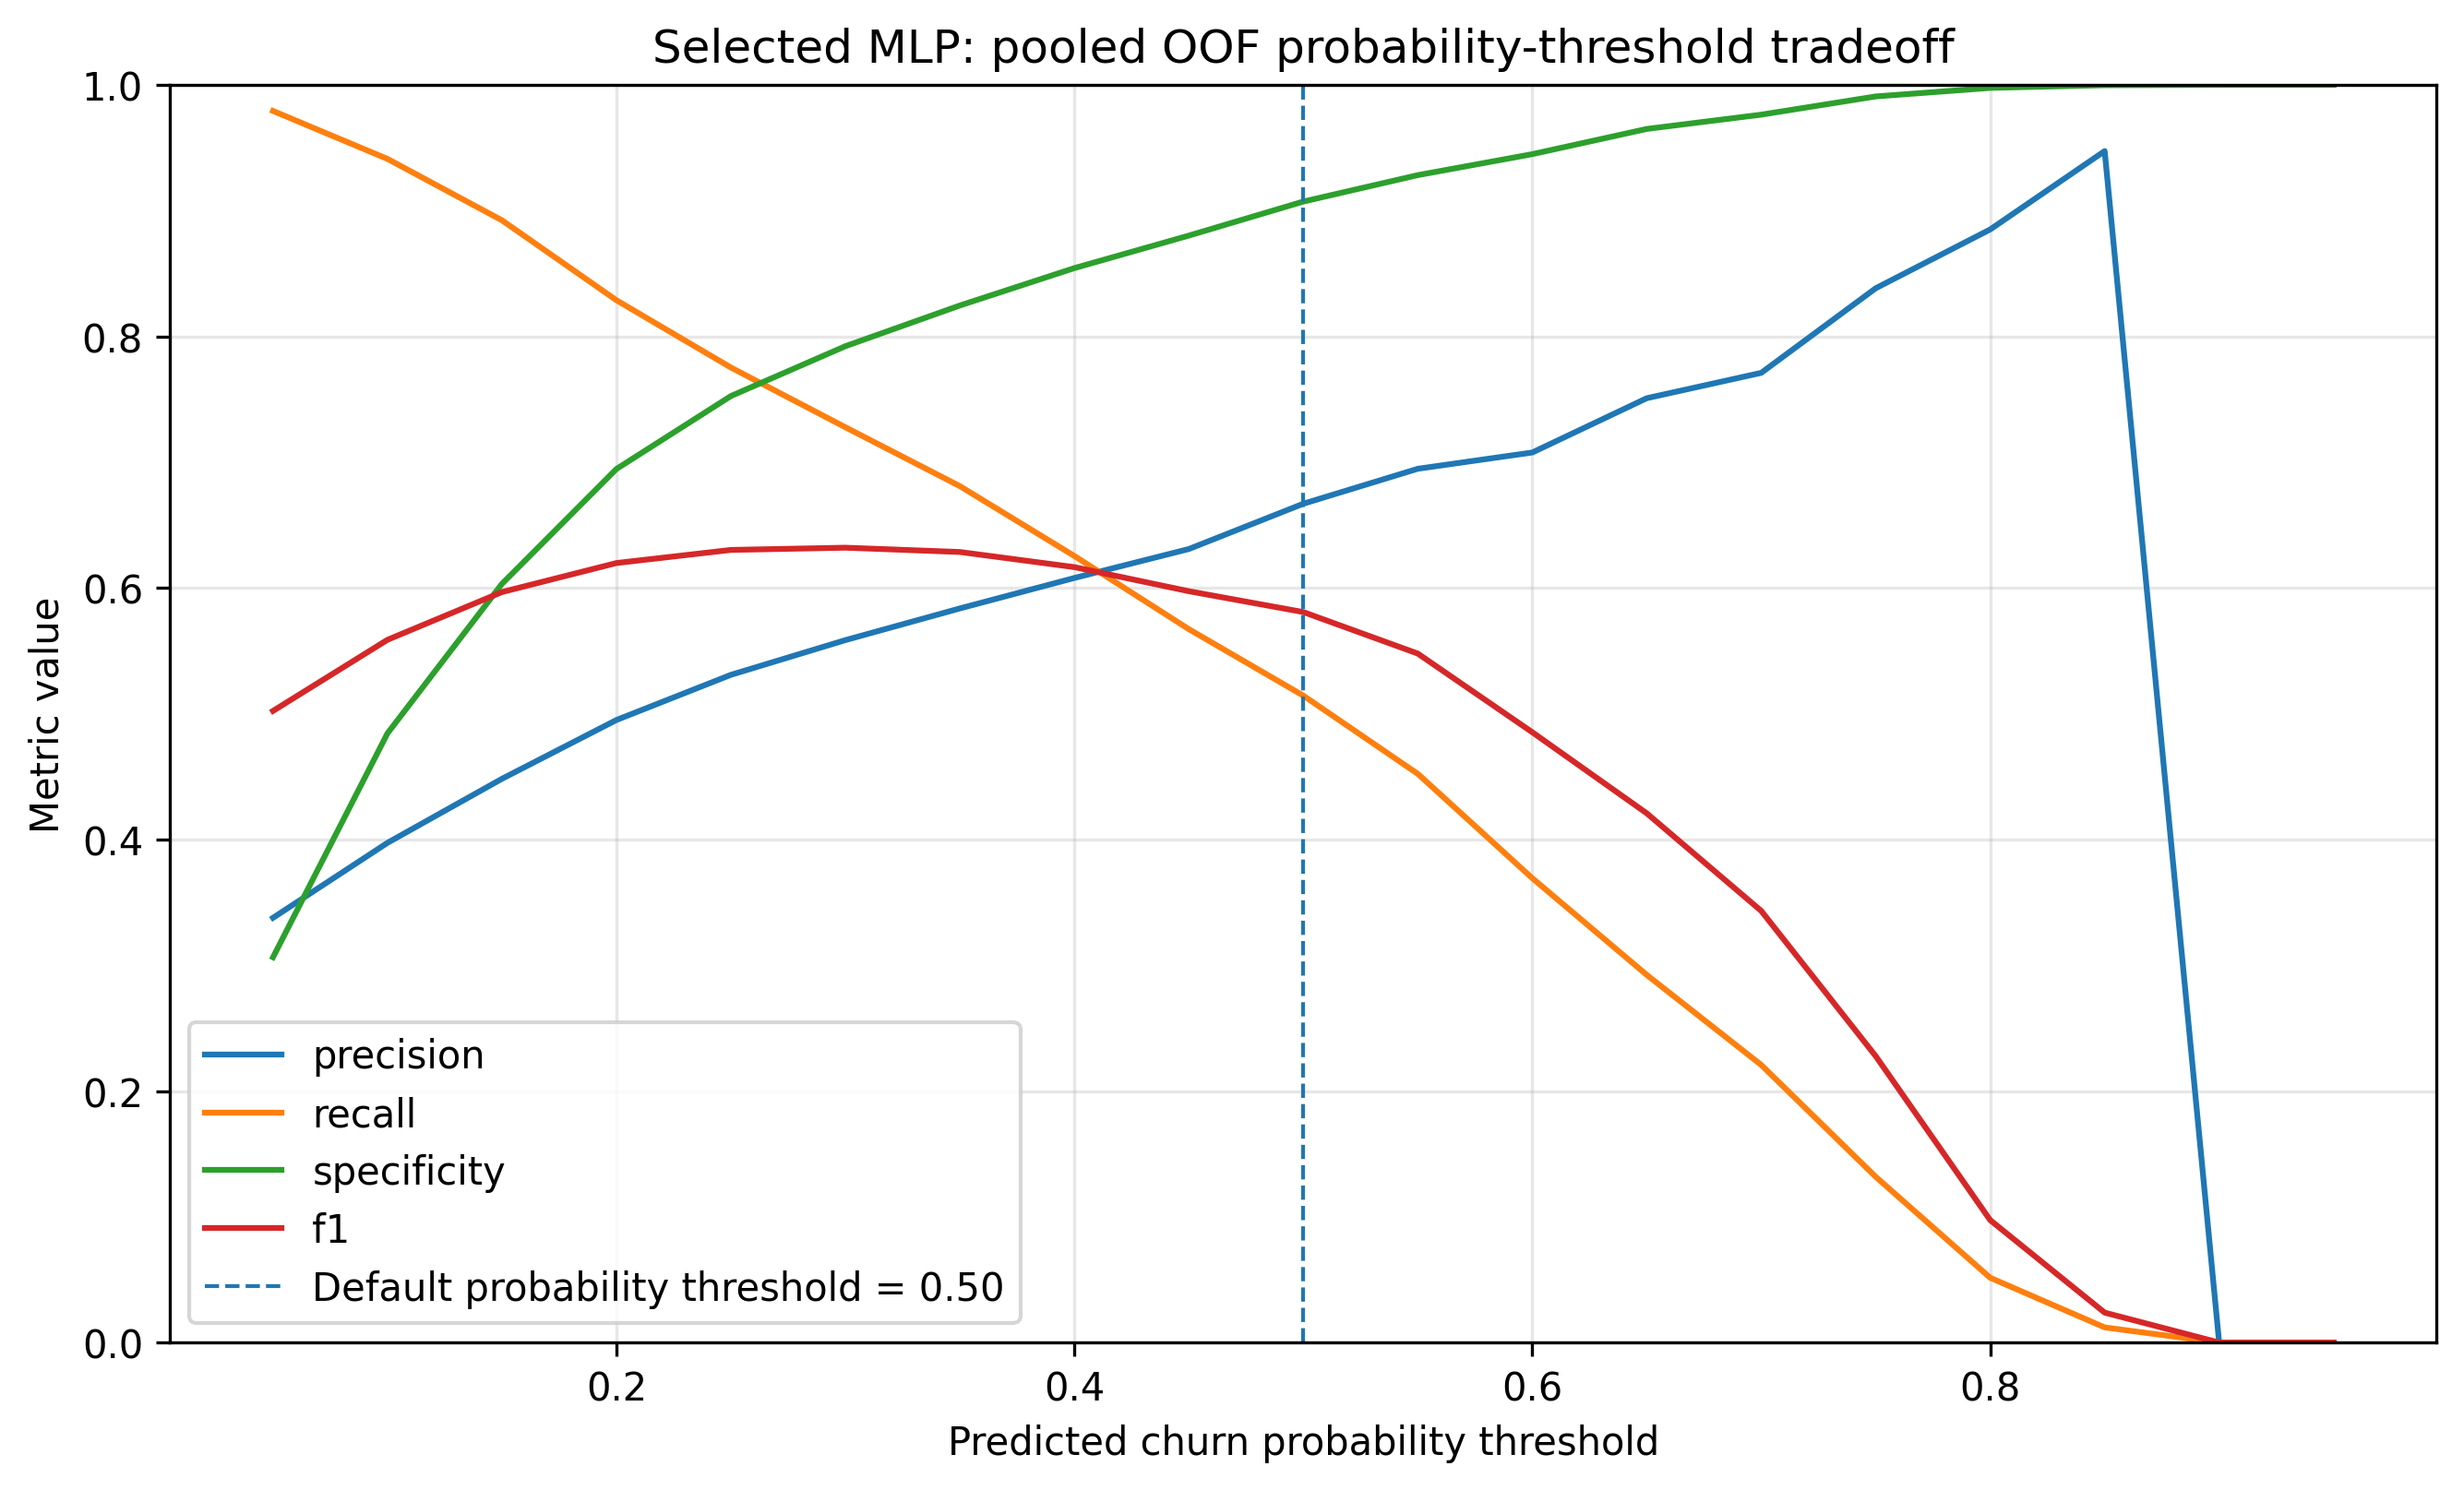
\includegraphics[width=0.88\textwidth]{../figures/mlp_probability_threshold_tradeoff.png}
\caption{Probability-threshold tradeoff for the selected MLP using pooled out-of-fold predictions}
\label{fig:mlp-threshold-tradeoff}
\end{figure}

\subsection{Calibration diagnostic}

The pooled OOF Brier score is \(0.1362\). For context, a non-informative predictor that assigned every customer the observed churn prevalence would have Brier score approximately
\[
\bar{y}(1-\bar{y})
=
0.265(1-0.265)
\approx
0.195.
\]
The selected MLP's mean predicted churn probability is \(0.2588\), close to the observed churn rate \(0.2654\). The ten-bin calibration curve is generally close to the ideal diagonal, although individual bins necessarily have sampling variability.

This is encouraging descriptive evidence, not a declaration that the model is fully calibrated for deployment. Calibration should later be compared systematically across serious finalists, and any calibration transformation must be estimated within a training-only resampling procedure.

\begin{figure}[H]
\centering
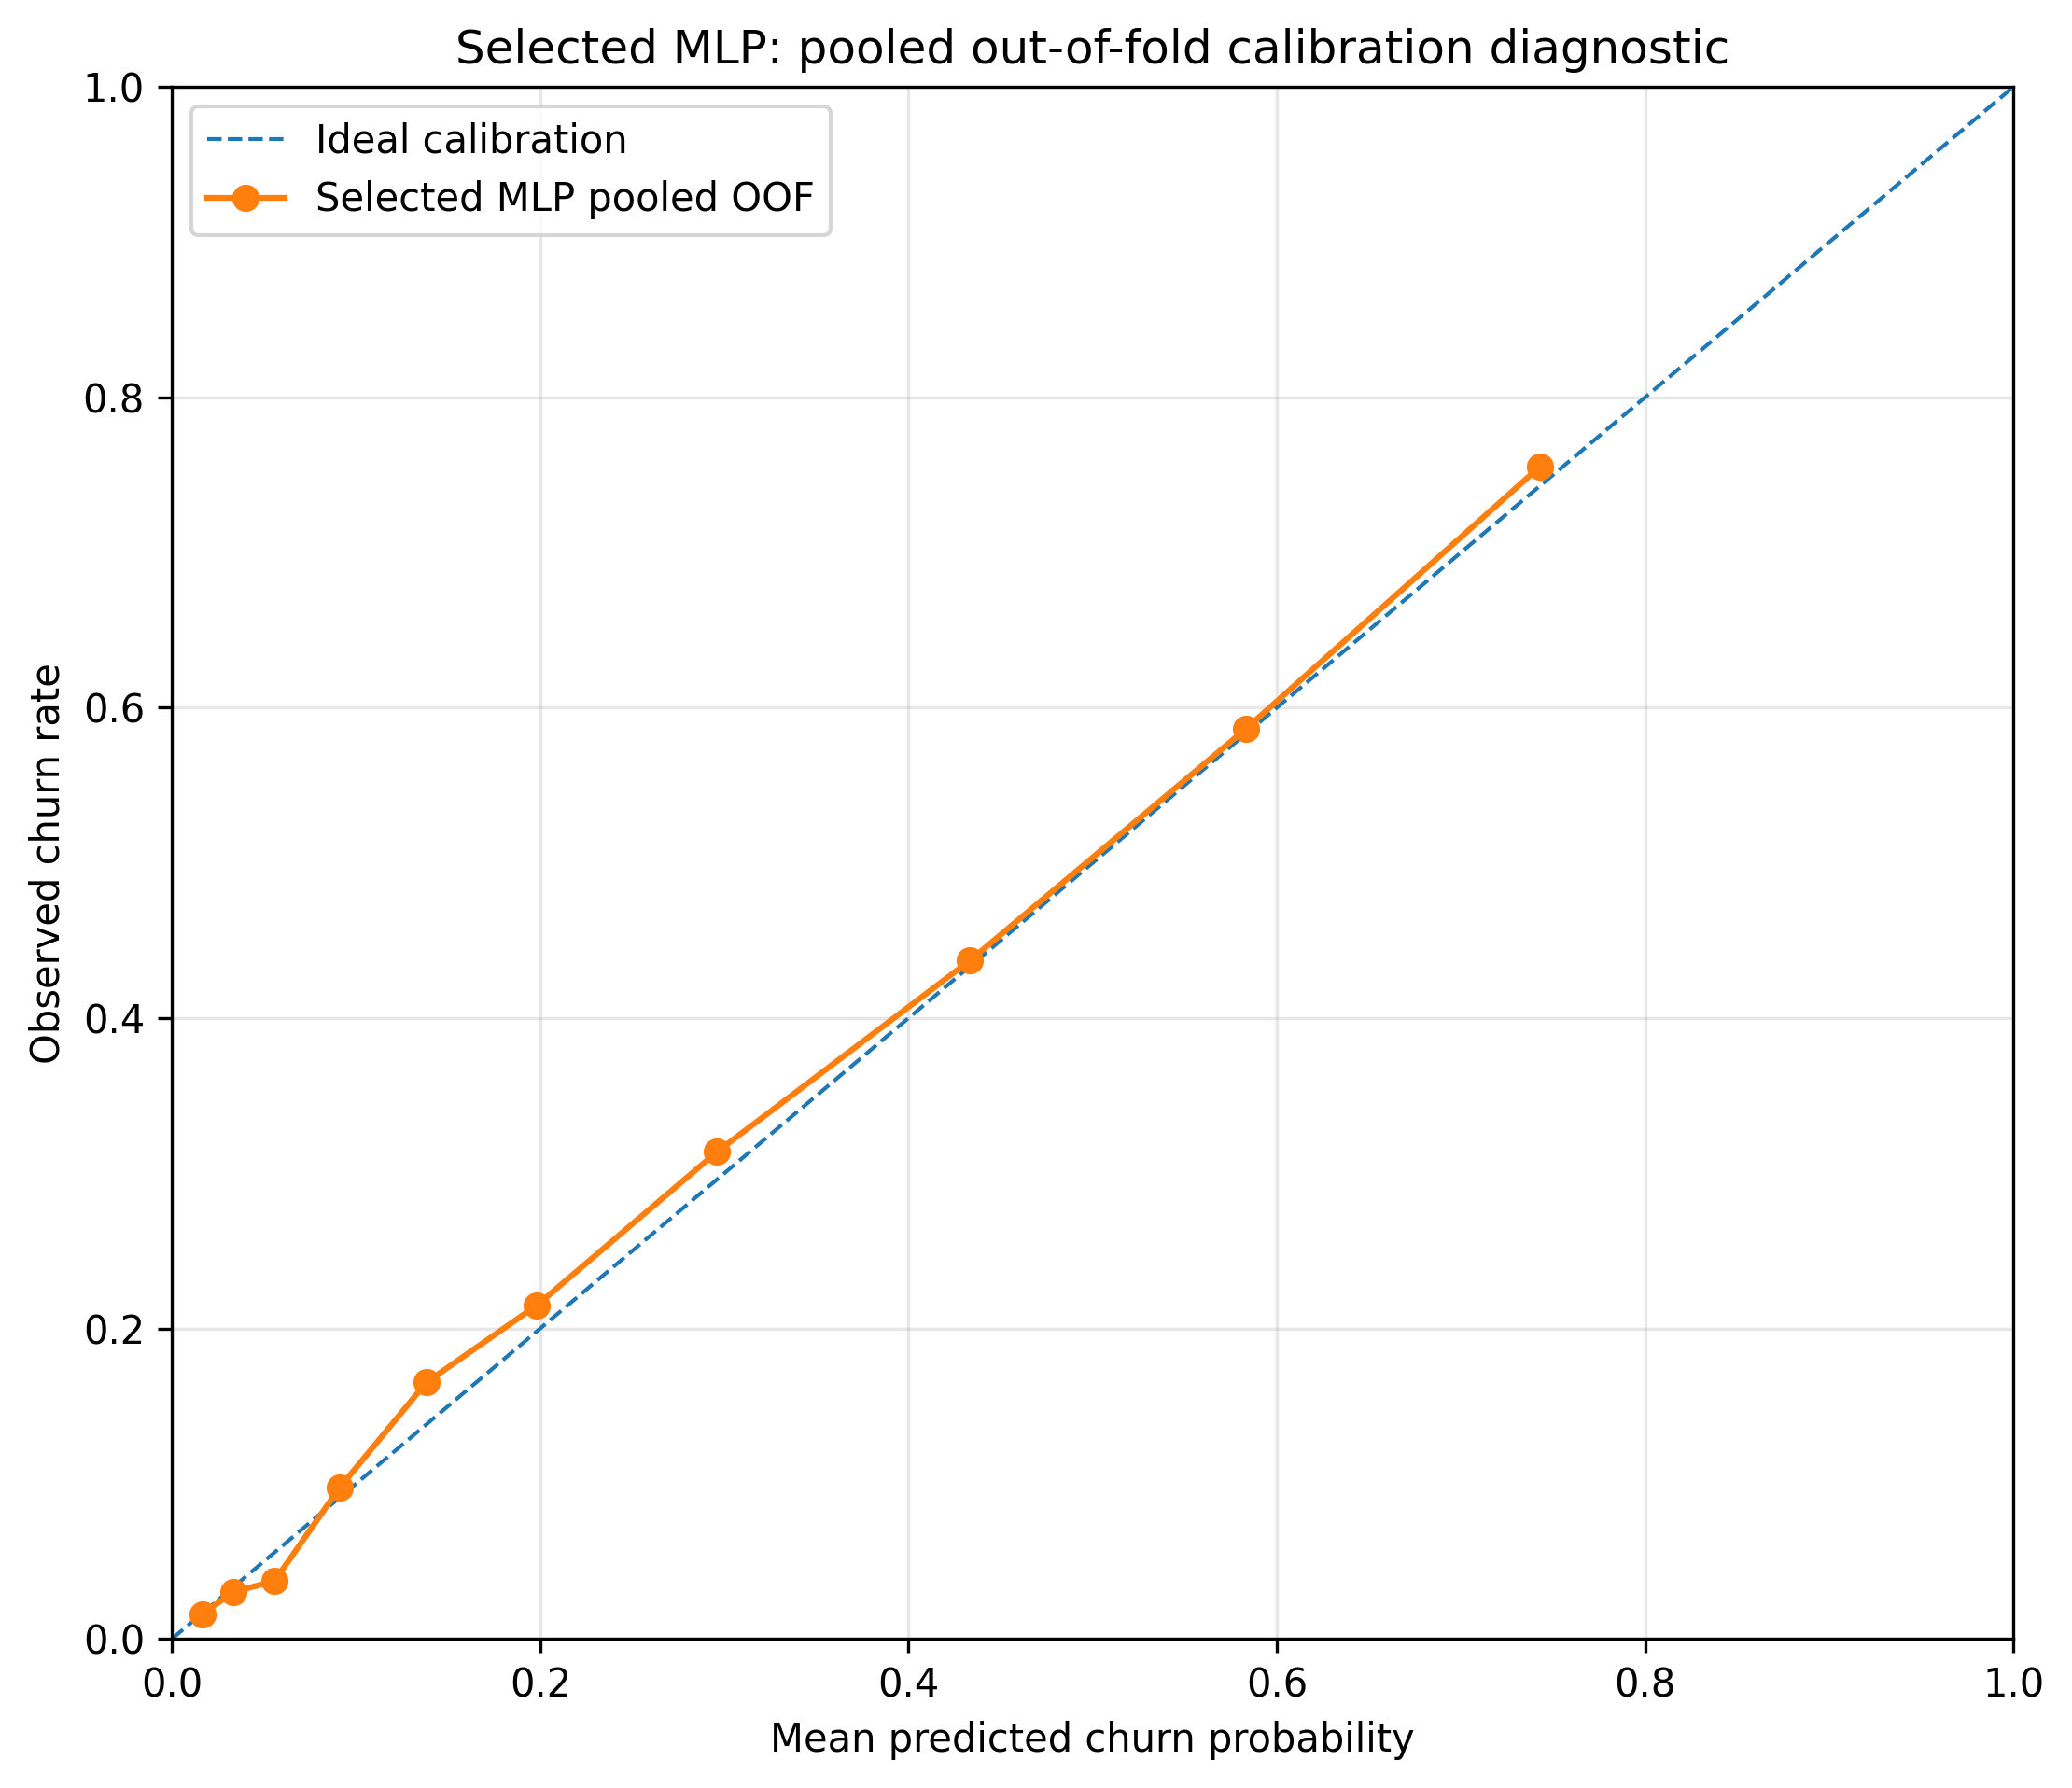
\includegraphics[width=0.82\textwidth]{../figures/mlp_calibration_curve.png}
\caption{Pooled out-of-fold calibration diagnostic for the selected MLP}
\label{fig:mlp-calibration}
\end{figure}

\subsection{Optimization and seed-sensitivity diagnostics}

When the selected pipeline is fitted once on the complete training set for optimization diagnostics, the training loss falls from approximately \(0.585\) in the first epoch to \(0.396\) after \(42\) epochs. The internal validation accuracy fluctuates around \(0.80\) and reaches a maximum of approximately \(0.811\). There are no convergence warnings in the five outer-fold fits or the full-training diagnostic fit.

The full-training curves are not independent performance estimates. Their role is to check that optimization is numerically stable, that the loss decreases, and that early stopping intervenes before a fixed \(500\)-iteration limit is exhausted. They must not replace the outer-fold validation metrics for model comparison.

\begin{figure}[H]
\centering
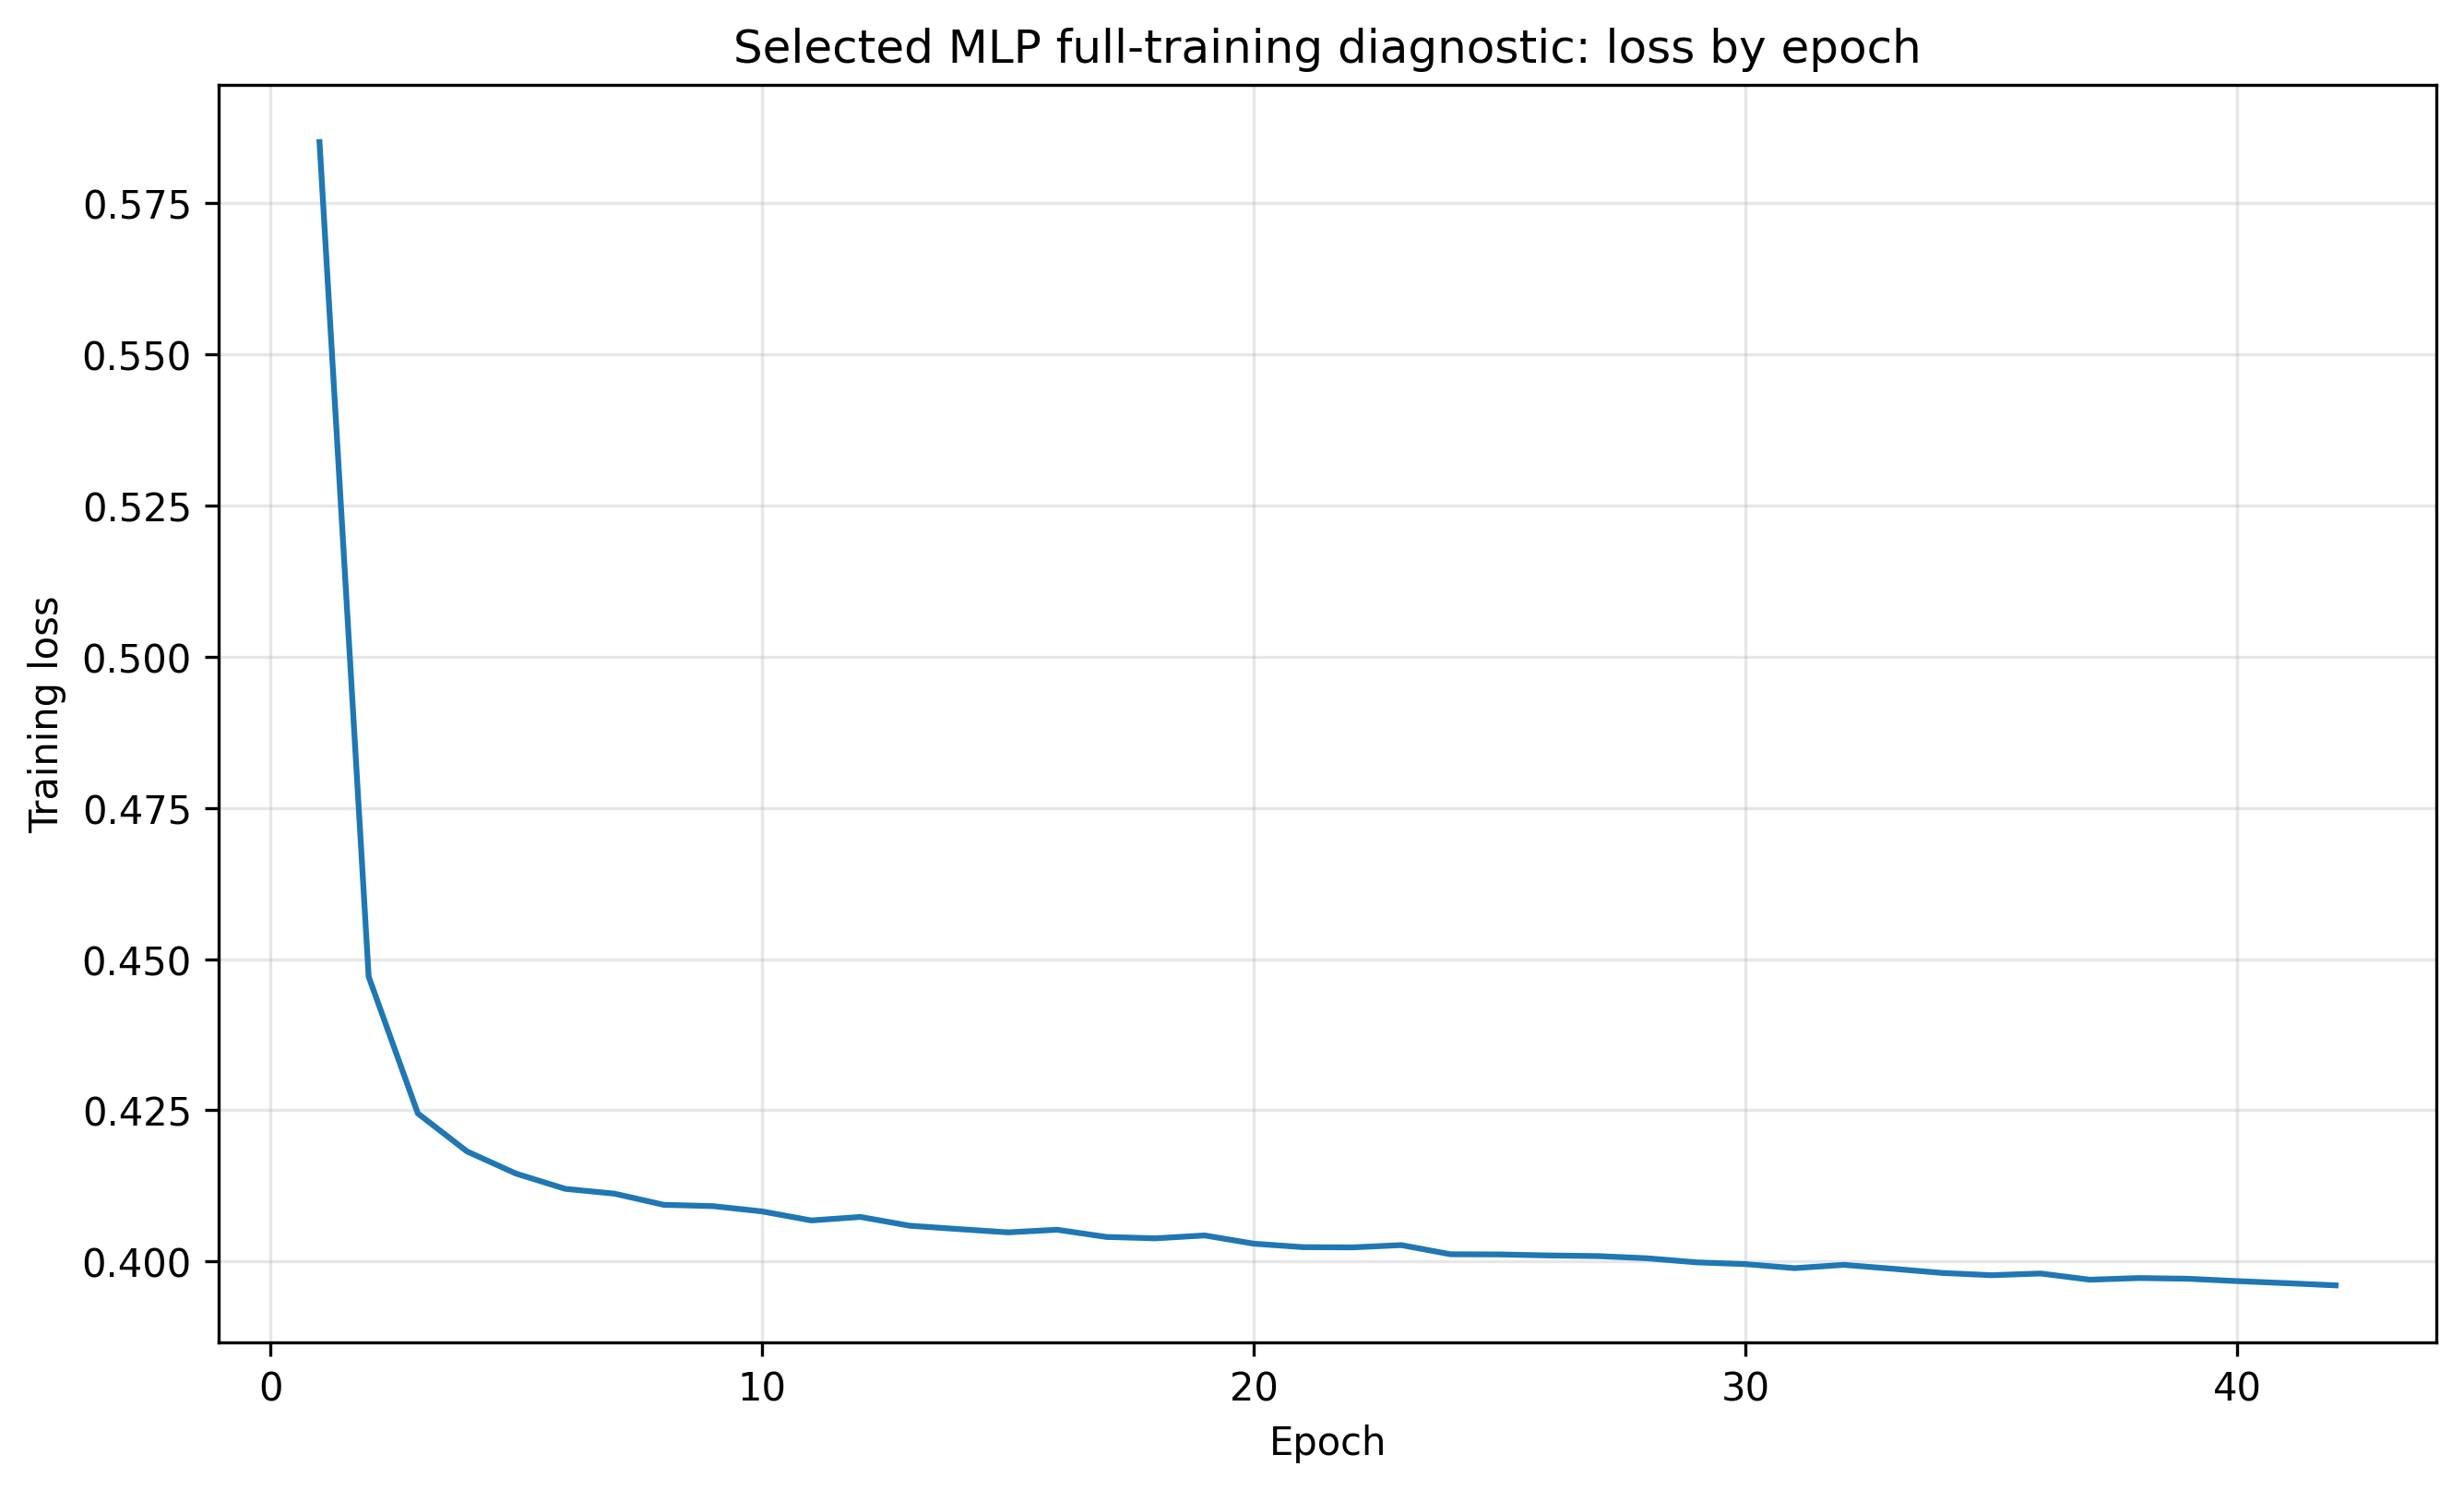
\includegraphics[width=0.82\textwidth]{../figures/mlp_training_loss_curve.png}
\caption{Full-training loss trajectory for the selected MLP diagnostic fit}
\label{fig:mlp-training-loss}
\end{figure}

\begin{figure}[H]
\centering
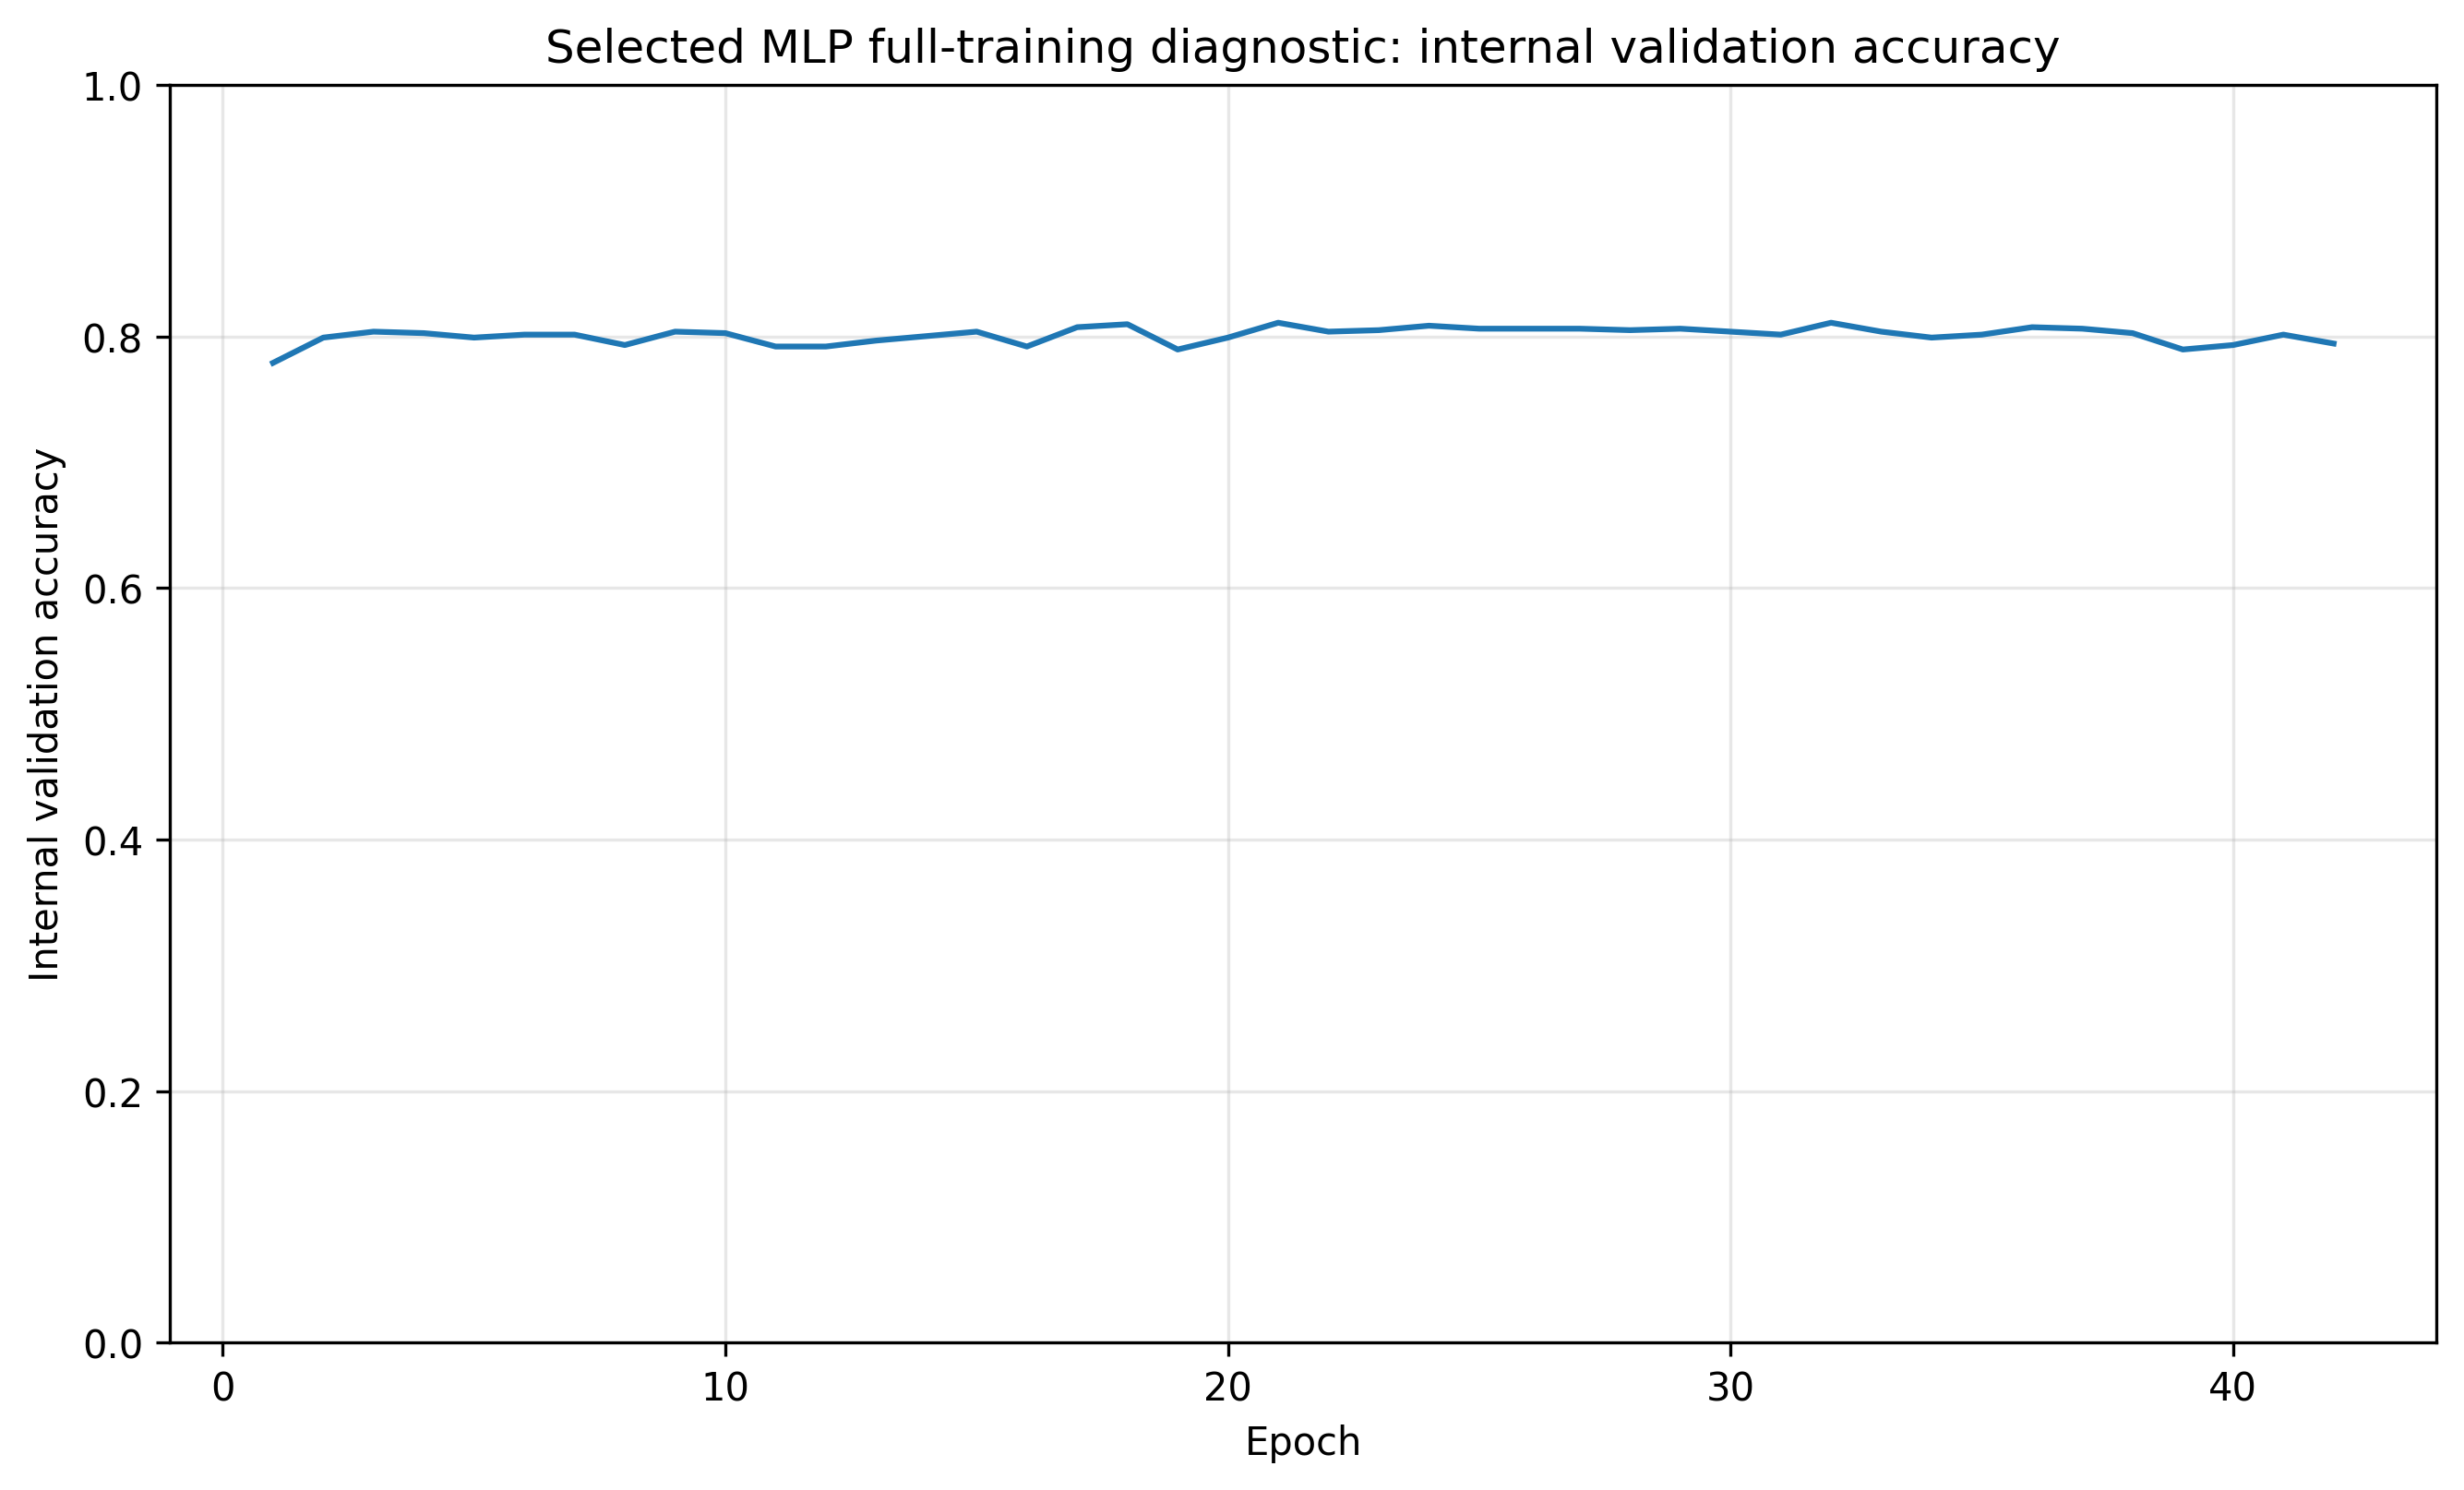
\includegraphics[width=0.82\textwidth]{../figures/mlp_internal_validation_accuracy_curve.png}
\caption{Internal validation-accuracy trajectory for the selected MLP diagnostic fit}
\label{fig:mlp-internal-validation}
\end{figure}

Neural-network fitting is stochastic because of random initialization and minibatch optimization. The selected architecture was therefore re-evaluated across four random states. Pooled OOF PR-AUC ranges from \(0.6502\) to \(0.6554\), with standard deviation approximately \(0.0023\). This is modest variation, but it is large enough to reinforce the general conclusion that small differences among nearby MLP grid configurations should not be treated as decisive.

\begin{figure}[H]
\centering
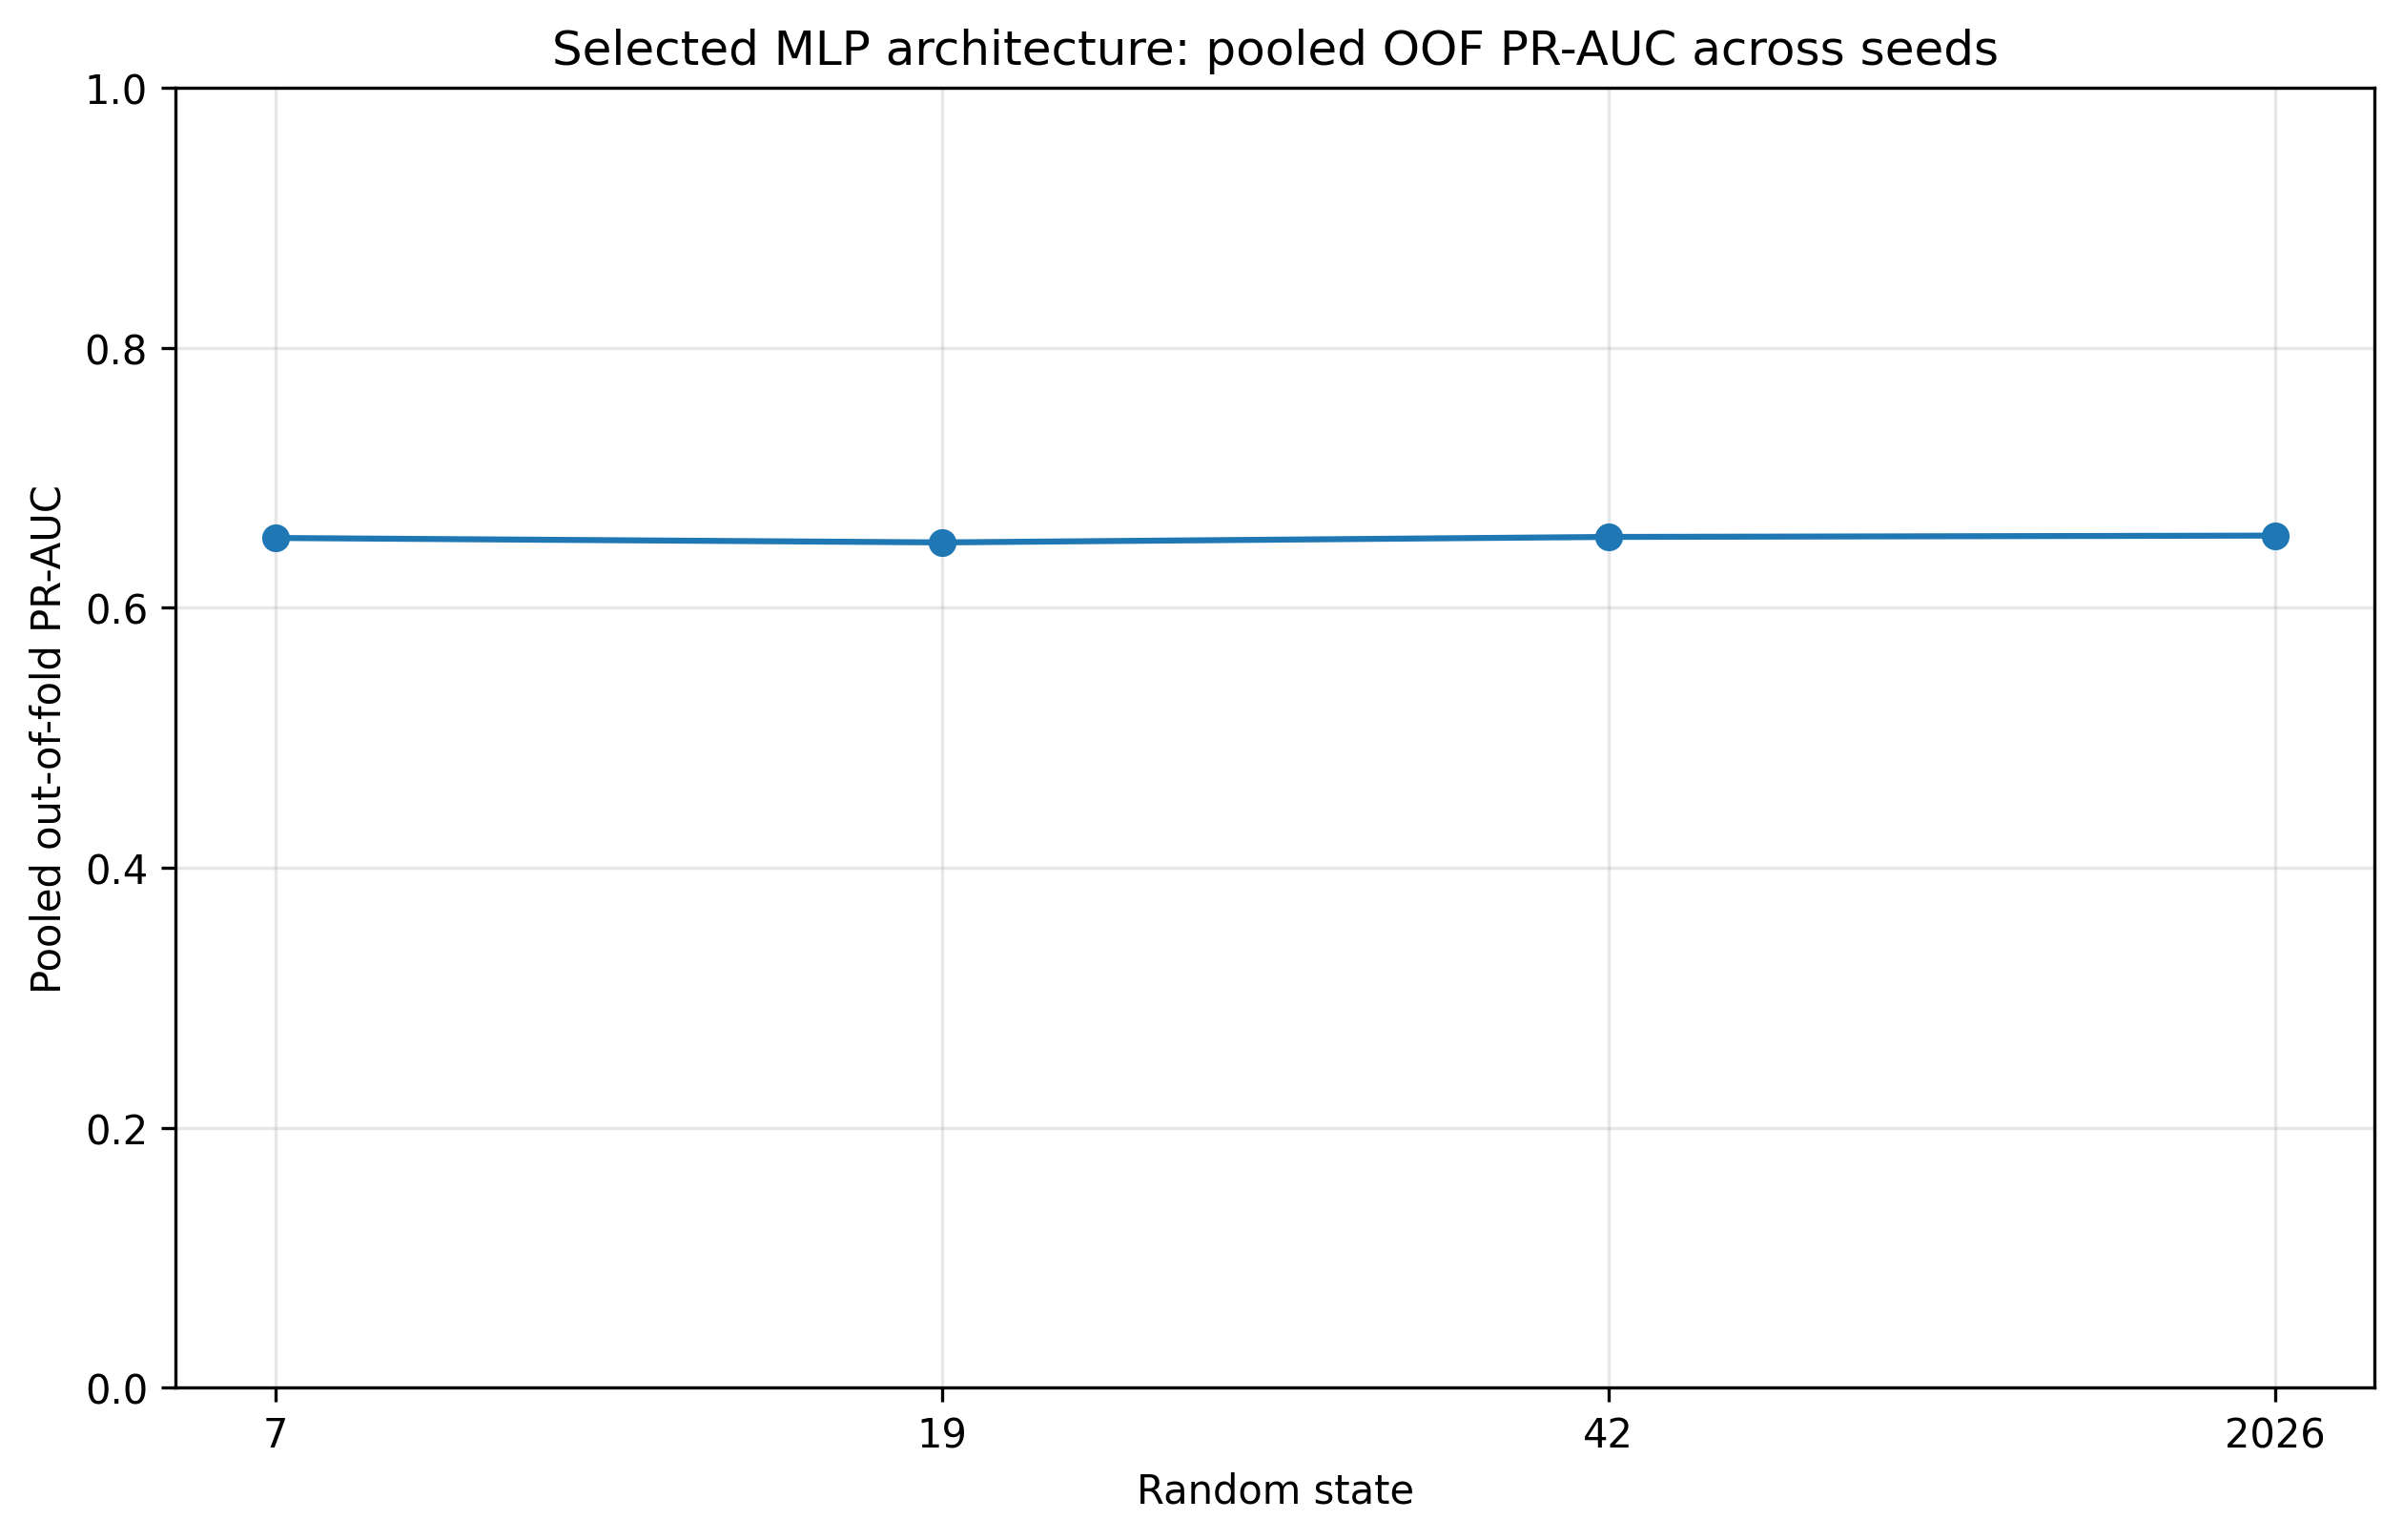
\includegraphics[width=0.82\textwidth]{../figures/mlp_seed_sensitivity_pr_auc.png}
\caption{Pooled OOF PR-AUC of the selected architecture across random seeds}
\label{fig:mlp-seed-sensitivity}
\end{figure}

\subsection{Scoped comparison with representative earlier models}

The MLP is compared with a deliberately limited set of earlier selected configurations. Each reference is reconstructed from the relevant earlier workflow and re-evaluated through fresh training-only cross-validation in the MLP notebook. This supplies comparable pooled OOF predictions and metrics under the same current pipeline and evaluation utilities.

Table~\ref{tab:mlp-model-comparison} is not a final project-wide ranking. It does not include all earlier boosting variants, random forest, RBF SVM, Naive Bayes, or every baseline. It is a local diagnostic that compares the MLP against representative linear, instance-based, single-tree, bagging, margin-based, and strong boosted-tree approaches.

\begin{table}[H]
\centering
\small
\resizebox{\textwidth}{!}{
\begin{tabular}{lrrrrrrrr}
\toprule
Model & Accuracy & Bal. Acc. & Precision & Recall & Specificity & \(F_1\) & ROC-AUC & PR-AUC \\
\midrule
Representative XGBoost & 0.808 & 0.722 & 0.671 & 0.539 & 0.905 & 0.598 & 0.850 & 0.670 \\
Selected bagged trees & 0.800 & 0.705 & 0.662 & 0.504 & 0.907 & 0.572 & 0.846 & 0.662 \\
Selected L2 logistic regression & 0.802 & 0.719 & 0.652 & 0.544 & 0.895 & 0.593 & 0.846 & 0.658 \\
Selected LinearSVC & 0.745 & 0.765 & 0.513 & 0.807 & 0.723 & 0.627 & 0.845 & 0.657 \\
Selected MLP & 0.803 & 0.711 & 0.667 & 0.514 & 0.907 & 0.581 & 0.842 & 0.654 \\
Selected decision tree & 0.789 & 0.701 & 0.624 & 0.514 & 0.888 & 0.564 & 0.824 & 0.628 \\
Selected kNN & 0.792 & 0.722 & 0.617 & 0.571 & 0.872 & 0.593 & 0.836 & 0.628 \\
\bottomrule
\end{tabular}
}
\caption{Scoped pooled out-of-fold comparison of the selected MLP and representative earlier models}
\label{tab:mlp-model-comparison}
\end{table}

In this scoped comparison, the selected MLP is competitive with the selected logistic regression and linear SVM in ranking quality, but it does not exceed the representative XGBoost, bagging, or logistic-regression references in PR-AUC. The MLP and XGBoost have similar default precision and specificity, but the XGBoost reference has higher recall and PR-AUC at its displayed default operating point.

The results therefore do not supply evidence that the MLP's learned nonlinear representation materially improves churn ranking beyond the strong existing approaches. That is a result about the evaluated architecture and search scope, not a claim that neural networks cannot work for churn prediction or tabular data in general.

\begin{figure}[H]
\centering
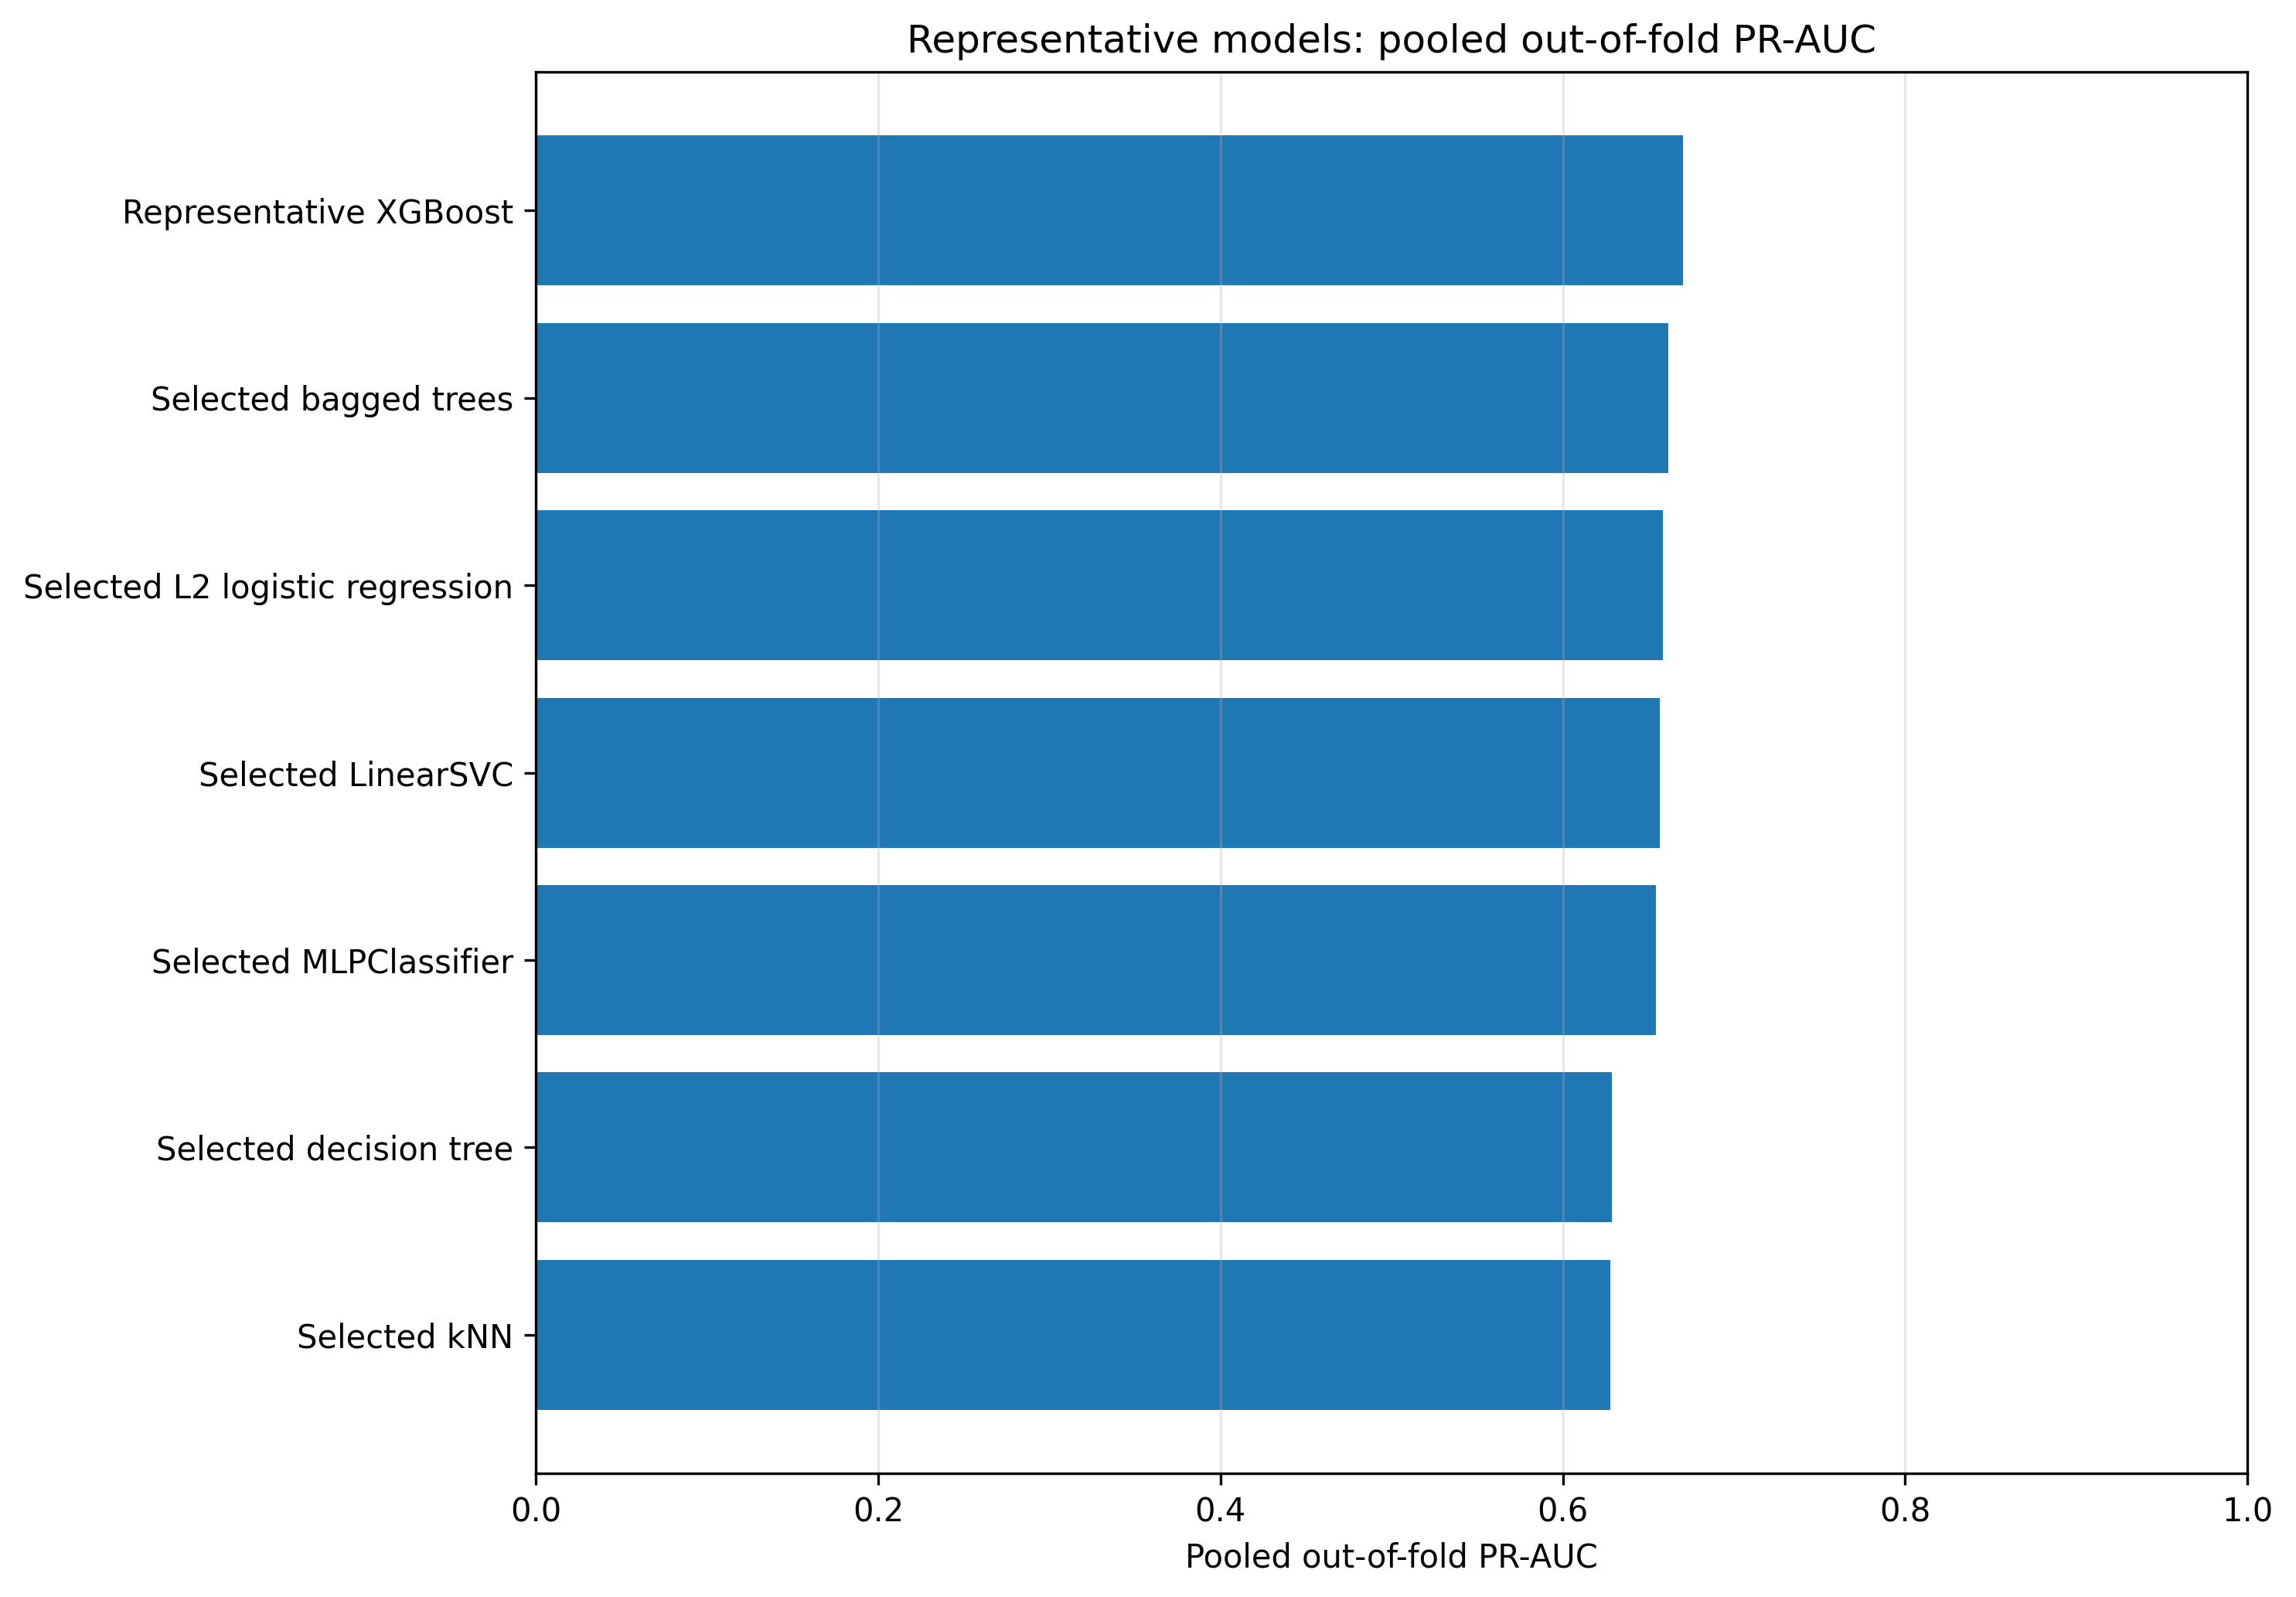
\includegraphics[width=0.90\textwidth]{../figures/mlp_model_comparison_pr_auc.png}
\caption{Selected MLP and representative earlier models: pooled out-of-fold PR-AUC}
\label{fig:mlp-model-comparison}
\end{figure}

\subsection{Conclusion and role in later selection}

The MLP workflow establishes a reproducible neural-network reference for the project: dense fold-safe preprocessing, a compact geometry-aware search, outer-fold PR-AUC selection, early-stopping diagnostics, probability-based threshold analysis, calibration inspection, and seed-sensitivity checks.

The selected \(16\)-unit ReLU MLP is a credible development-stage candidate with useful discrimination and reasonable pooled OOF calibration behaviour. However, the compact search does not demonstrate a clear advantage from additional width, depth, or a \(\tanh\) activation, and the scoped comparison does not show a material ranking advantage over the strongest earlier references.

No final model is selected in this section. A later finalist workflow should define a serious candidate set, compare frozen procedures fairly with appropriate uncertainty assessment, assess calibration where required, choose an operating threshold using retention economics and contact capacity, fit one frozen pipeline on the complete training set, and evaluate the held-out test set once.
